\cleartoevenpage
\pagestyle{empty}	%Use this to suppress the header from the preceding chapter.


\begin{table}[h]
	\begin{center}
	\begin{tabular}{|c|l|l|}
		\hline
		Contributor & Statement of contribution & \% \\
		\hline
		\textbf{Edward M. Barry}	    & writing of text 			& 80\\
										& proof-reading				& 60 \\
										& theoretical derivations 	& 50 \\
										& numerical calculations 	& 100\\
										& preparation of figures 	& 100 \\
										& initial concept			& 30 \\
		\hline
		Christopher T. DeGroot			& writing of text 			& 0\\
										& proof-reading				& 5 \\
										& supervision, guidance 	& 15\\
										& theoretical derivations 	& 10\\
										& preparation of figures 	& 0 \\
										& initial concept			& 0 \\
		\hline
		Shakil Ahmmed       			& writing of text 			& 10\\
										& proof-reading				& 0 \\
										& supervision, guidance 	& 25\\
										& theoretical derivations 	& 40\\
										& preparation of figures 	& 0 \\
										& initial concept			& 0 \\
		\hline
		Tim H\"{u}lsen		    		& writing of text 			& 0 \\
										& proof-reading				& 0 \\
										& supervision, guidance 	& 10 \\
										& theoretical derivations 	& 0 \\
										& preparation of figures 	& 0 \\
										& initial concept			& 35 \\
		\hline
		Damien J. Batstone	    		& writing of text 			& 10\\
										& proof-reading				& 95 \\
										& supervision, guidance 	& 50 \\
										& theoretical derivations 	& 0 \\
										& preparation of figures 	& 0 \\
										& initial concept			& 35 \\
		\hline
	\end{tabular}
	\end{center}
\end{table}


%-------------------------------------------------------------------------------------------------------%
%-------------------------------------------------------------------------------------------------------%
%-------------------------------------------------------------------------------------------------------%
%-------------------------------------------------------------------------------------------------------%
%-------------------------------------------------------------------------------------------------------%
%-------------------------------------------------------------------------------------------------------%
%This is an internal chapter of the thesis.
%If you have a long title, you can supply an abbreviated version to print in the Table of Contents using the optional argument to the \chapter command.
\chapter[A multidimensional phototrophic biofilm model]{A multidimensional, phototrophic, continuum-based biofilm model}
\label{chap:ch4}	%CREATE YOUR OWN LABEL.
\pagestyle{headings}

\section*{Abstract}
Phototrophic bacteria have an ability to remove soluble organics and nutrients from waste streams while at the same time producing products of high value such as pigments, biocrude, high protein feedstock. 
However, phototrophic and photosynthetic systems are critically dependent on light delivery and biomass harvesting to remove organics and nutrients from the process.
No substantial work to date has been done on modelling photo-dependent biofilm growth.
This study aims to develop a multidimensional continuum-based phototrophic biofilm model to serve as a basis for exploring the physical mechanisms associated with photobiofilm formation and for potential process optimisation. 
A volume of fluid (VoF) model in which phototrophic biomass could be grown on a substratum was developed. 
This evaluates the interactive mechanisms of substrate transport and radiative attenuation through the bulk and biofilm. 
Investigating coupling between the biofilm and the radiative field was the major motivator of the study. 
The lamp source was set from below and above the biofilm on both uniformly and sparsely initiated biofilms at 30 W m\textsuperscript{-2}. An extra simulation was done where the lamp source was set at 10\% intensity and placed below the biofilm. In all cases, there was phototrophic growth, however in the case of minimal irradiation, the maximum growth rate was 70\% slower than the case with 30 W m\textsuperscript{-2}. 
Maximum growth rate was 25\%-30\% slower in the cases where the radiative intensity field was initiated from above the biofilm, due to liquid attenuation. This was despite the decreasing substrate diffusion limitations. 

%This model provides a basis for a multispecies, multidimensional phototrophic biofilm model which accounts for all physical phenomena in the life-cycle of the biofilm, however experimental work is required to calibrate the model for a non-planktonic case.
%-------------------------------------------------------------------------------------------------------%
%-------------------------------------------------------------------------------------------------------%
%-------------------------------------------------------------------------------------------------------%
\section{Introduction}
Despite a growing interest in the use of purple phototrophic bacteria (PPB) for wastewater treatment and the production of high valued products, there remain key engineering challenges which render widespread adoption in full scale installations unfeasible at this moment.
The major challenges have already been discussed throughout this thesis, but to reiterate, light delivery, the additional requirement of bioavailable organics, and solid-liquid separation are some of the major barriers \cite{hulsen2016}. 
Process modelling is an important tool for a better understanding of how phototrophic processes work, and for eventual process design and optimisation. 
Indeed, this thesis is based on the modelling of these phototrophic processes using the distributed parameter approach of computational fluid dynamics (CFD). 
This work has built upon the development of a biokinetic model, where the main metabolic processes were defined in a manner that ensured compatibility with the International Water Association family of models (IWA) such as the anaerobic digestion model 1 (ADM1) \cite{batstone2002} or the ASM models \cite{henze2000}. 
The biokinetic process model was extended to include dynamics in multidimensional space in order to demonstrate the spatially varying nature of the radiative field, and by extension, the growth of phototrophic biomass. 
In addition to organics and radiative field limitations, the third constraining factor is the separation of the solid phototrophic biomass from the liquid phase. 
Previously, anaerobic membrane bioreactors were proposed as a solution for solid-liquid separation at laboratory-scale implementations \cite{hulsen2016}, however with increased capital and operational expenditure when compared to conventional wastewater treatment processes, more separation techniques need to be explored. 
Growing biomass attached to walls as biofilm can be a method to reduce harvesting costs of phototrophic biomass, as well as reducing inefficient delivery of light due to the self shading associated with biomass growth. As such, a phototrophic biofilm model in a CFD framework needs to be developed. 
\skippingparagraph
Phototrophic biofilms are communities of phototrophic biomass, other organisms, and other organic and inorganic substances such as extra-cellular polymeric substances \cite{vanloosdrecht2002}. 
Much work has been dedicated to understanding the behaviour of biofilms in order to limit the harm they cause, such as in medical settings, sewer networks \cite{pikaar2014}, and in membrane separation processes, commonly referred to as fouling \cite{radaei2018}. Biofilm formation can also be favoured and encouraged depending on the application. 
Trickling filters are an example of beneficial biofilms which consist of wastes being sprayed over fixed granular beds. Thick biofilms develop therein and remove pollutants and toxicants from the filter's biofilm \cite{donlan2002}. Other examples of beneficial biofilms include the bioremediation of contaminated soils \cite{singh2006}, which claim an advantage over biological treatment with planktonic cells in that microorganisms in biofilms are more resilient to extreme conditions, and therefore have a better chance at adapting to their particular environment. Biofilms may grow on a physical substrate (moving or fixed media), or be self supporting in the form of anaerobic or aerobic granules \cite{baeten2018}. 
\skippingparagraph
In order to successfully model biofilm formation and behaviour, the governing processes need to be identified. The major processes are the initial attachment, biofilm growth, biofilm decay, and detachment \cite{alpkvist2007}. 
These processes have been represented by several modelling approaches. The approaches are divided into first, second and third generation models as defined by the IWA task group on biofilm modelling \cite{wanner2006}. 
The progress from first to third generation has seen the modelling approach evolving from mass transfer to the inclusion of complex microbial interactions and an update to two and three dimensional descriptions. First generation models involved the description of substrate gradients (mostly a single limiting substrate) within an homogeneous 1-dimensional zone of biomass. Second generation models differed from their predecessors in that they included multiple substrates and microorganisms in a heterogeneous distribution. They were still limited to a 1-dimensional description. 
Third generation models represent particulates as discrete elements, a continuum field, or a combination of both. Discrete biofilm models include cellular automata and agent based models \cite{skoneczny2015}. 
With discrete techniques, cells are subjected to a set of rules that govern their behaviour in terms of attachment, substrate uptake and cell division, and decay and detachment processes \cite{skoneczny2015}. 
These models are relatively simple to develop, however simulation cycles require statistical rigour and multiple simulation runs, as the aggregate effect of individual particles can result in artefacts, which need to be assessed by averaging multiple runs (or very large numbers of discrete elements) \cite{dacunto2017}. 
In contrast to discrete third generation biofilm models, continuum-based models involve a full spatio-temporal and mechanistic description of biofilm processes \cite{eberl2001}. 
An advantage of continuum-based biofilm models over discrete approaches is that a mechanistic description of growth processes can be developed into the model.
Biokinetic models such as the Eilers-Peeters model for algal growth \cite{eilers1988} or the PAnM1 model \cite{puyol2017} can therefore be used directly within a phototrophic biofilm modelling framework, albeit with some manipulations to convert the model from a COD or equivalent basis, to a volumetric growth basis. 
\skippingparagraph
Despite the increasing interest in phototrophic bioreactors, and the motivation to better control photobiofilm development, there are only two clear examples of phototrophic biofilm modelling. 
The first continuum-based biofilm model \cite{clarelli2013} identified the non-conservative nature of interface evolution tracking methods such as the level-set method \cite{alpkvist2007} and proposed a mixture model for cyanobacterial biofilms. 
The mixture model treats each point in space as an information holder, in which multiple physical properties and states can exist. 
This mixture model provided a mathematical description of a specific case of a cyanobacterial biofilm which according to the authors could be extended to all phototrophic biofilm systems. 
This study presented an exponential decay function for the radiative field through the biofilm, which has a tendency to under predict the radiative distribution for optically thick media such as biofilms \cite{jarosz2008}. 
In optically thick media, strong scattering effects are observed, including forward scattering \cite{jarosz2008}. 
This phototrophic/photosynthetic biofilm mixture model was further developed in subsequent studies \cite{polizzi2017}. In this study a single functional microbial group (microalgae), its associated carbon pool, and an extra-cellular polymeric matrix were all defined as biofilm components. CO\textsubscript{2}, O\textsubscript{2} and inorganic nitrogen formed the liquid component of the model. Mass transfer between phases was updated to include diffusion terms, and biofilm expansion was expressed in terms of biological mechanisms such as photosynthesis, cell maintenance, EPS excretion and cell decay. 
The radiative field was also modelled as an exponential decay function in terms of path length and the concentrations of participating biofilm components.
\skippingparagraph

The proposed model in this work differs from the previous PBF examples in the following aspects:

\begin{enumerate}
\item Biofilm models should be developed for implementation in all spatial dimensions. Decisions to simplify the model should be made by the user at implementation. Presented here is a multidimensional phototrophic biofilm model.
\item The evolving structure of the biofilm must be captured. The advancement of the biofilm front is coupled to biomass growth and decay processes. The interface between biofilm and liquid is captured by a conservative, coupled volume-of-fluid (VoF) and level-set method.
\item Biofilms are heterogeneous in nature. Scope must be made to model multispecies biofilm evolution. As such, presented here is a multidimensional,  multispecies, dynamically structured phototrophic biofilm model.
\end{enumerate}

In addition to these three points of novelty, the biofilm model has been implemented in OpenFOAM, a computational fluid dynamics (CFD) finite volume method (FVM) framework. This package is a collection of C++ libraries which allow for the resolution of continuum mechanics problems. The model extends on previous work by the authors \cite{puyol2017}. The global purpose of this study is to explain the physical phenomena occurring within biofilms so that subsequent studies can progress the work for design or prediction purposes.

This study therefore aims to extend the previous work done on the development of a lumped parameter model in chapter 2, and of a phototrophic CFD model in which a coupled photo-biological radiative transfer model and planktonic growth model were defined in chapter 3. A combination of the volume of fluid (VoF) and mixture methods are used in this work: the VoF method to segregate the biofilm from the liquid phase, and the mixture method within the biofilm to differentiate between active phototrophic biomass (PPB  in this case), biodegradable particulates (X\textsubscript{S}) and inert particulates (X\textsubscript{I}). This method allows for conservation to be maintained while more accurately capturing the interface between the liquid and biofilm phases. 


%As biofilms are spatially heterogeneous structures, both spatial and temporal variations must be considered in order to describe the physical phenomena. Biofilm models can be divided into three main classes: \textit{i)} one-dimensional models capable of including mass transfer, reaction/diffusion, and detachment processes \cite{horn2014}, \textit{ii)} multidimensional discrete biofilm models such as cellular automata and agent based methods \cite{wang2010}, and \textit{iii)} continuum models including computational fluid dynamics (CFD) approaches \cite{alpkvist2007, duddu2009, cunault2015}. Despite the vast suite of modelling approaches and examples existing within the literature, there have been few studies which defining biofilm behaviour in phototrophic systems, where the spatially varying nature of the radiative field could be an important factor in the heterogeneous formation of biofilms. \\

%Representing biomass as continua can be advantageous. Firstly, the currency of process engineering modelling is differential balance equations. Continuum modelling is therefore a common language for communication of model development and results, and additionally, conservation of differential states can be ensured. In contrast to discrete modelling methods, deterministic solutions can be obtained for continuum-based models \cite{dacunto2017}. Difficulties can arise when modelling continuum-based biofilms. The frequently abrupt density jumps across liquid/solid boundaries can lead to numerical instabilities. The coupling of the non-linear transport equations with growth kinetics can also be problematic. Additionally, solving state equations with vastly different time constants (and order of 10s of seconds for fluid flow in a reactor, to hours or days for biomass growth and decay expressions) can make the resolution of the time discretisation difficult. Differential algebraic equations, or appropriate time discretion algorithms for stiff systems of differential equations can overcome this barrier. Computational fluid dynamics (CFD) packages can assist with some of the numerical problems and the mathematical formulation difficulties associated with continuum models.


% \begin{itemize}
% \item Biofilms are communities of microorganisms, EPS matrices and inert substances living together
% \item There are extrinsic properties leading to their growth:
% \begin{itemize}
% \item fluid flows
% \item irradiance
% \item presence of nutrients
% \item presence or absence of other microorganisms
% \item shear rates
% \item reactor geometry and operating conditions (implicitly)
% \end{itemize}
% \end{itemize}

%%%% PROBLEM DESCRIPTION
%\newpage
%\section{Problem description}
%\label{S:problem_description}
%The modelling approach is concerned with the description of a phototrophic biofilm system consisting of purple phototrophic bacteria (PPB). The model description for this system has been previously described \cite{puyol2017}, however this did not account for spatial variations, and by extension, biofilm formation was not considered. The phototrophic biofilm grows attached to a surface substratum. Above the biofilm is a body of nutrient-rich liquid. Incident photons of wavelength 850 \si{\nano \metre} are irradiated from either \si{\Gamma_0} or \si{\Gamma_3} into the domain \si{\Omega}, as shown in Fig. \ref{fig:2d_above}. The initial thickness of the biofilm is \SI{50}{\micro \metre} with uniformly distributed solid species. The factor of incident irradiance is also explored, with three different irradiance levels of \SI{10}{\watt \metre ^2}, \SI{30}{\watt \metre ^2}, and \SI{100}{\watt \metre ^2} being simulated from the surface substratum. Incident irradiance in all cases is assumed uniform and diffuse across the whole boundary.


% The phototrophic biofilm (PBF) model based on purple phototrophic bacteria is an extension of the models presented previously \cite{puyol2017} (\textbf{include my model}). Biofilm treatment extends work previously carried out by \cite{alpkvist2007}, \cite{alpkvist2007}. The important physical processes identified are as follows:
% \begin{itemize}
%     \item Coupled volume of fluid and level set for capturing of the biofilm/liquid interface.
%     \item Radiative transfer coupled to the growth of the biokinetics.
%     \item Biokinetics equations coupled to the radiative transfer equation (RTE) and the biofilm advection terms.
%     \item Development of a biofilm front velocity based on the evolution of pressure due to solid species growth within the biofilm.
% \end{itemize}


%\begin{figure}[htpb]
%    \centering
%    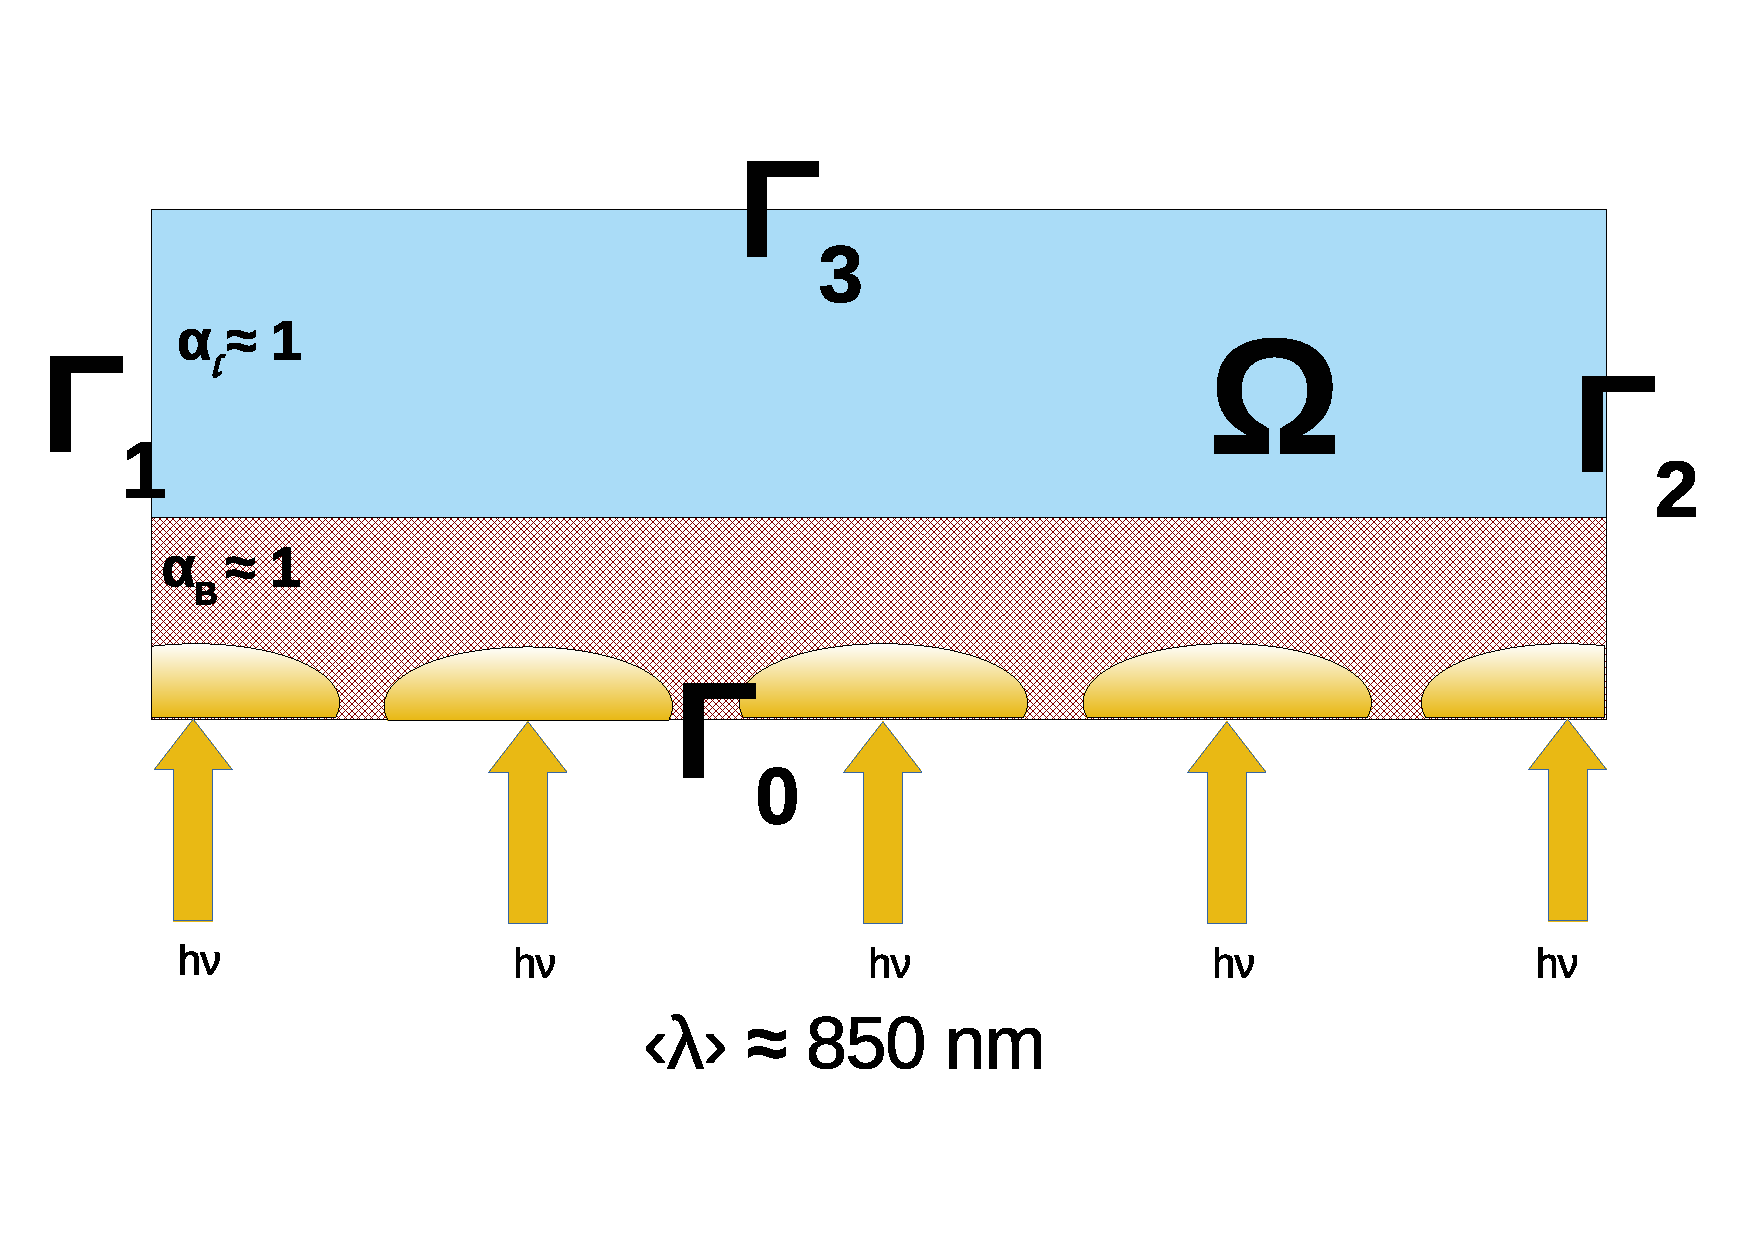
\includegraphics[scale=0.5]{Images/Chap4/prob_diagram_below.pdf}
%    \caption{Two-dimensional representation of the simulation domain for the case of a bottom-irradiated biofilm. Boundaries \si{\Gamma_4} and \si{\Gamma_5} are out of, and into the page respectively, and take the same boundary conditions as boundaries \si{\Gamma_1} and \si{\Gamma_2}. The irradiance source (\si{h \nu}) is in fact uniform and diffuse across the whole boundary. Subscripts relating to \si{\alpha}, namely \textbf{l} and \textbf{B} correspond to liquid phase fraction, and biofilm phase fraction respectively.} 
%    \label{fig:2d_above}
%\end{figure}


%%%%%%%%%%%%% MATHEMATICAL FORMULATION

\newpage
\section{Mathematical formulation}
\label{S:formulation}
\subsection{Radiative transfer}
The general form of the radiative transfer equation (RTE) has been adapted to phototrophic systems, presented in the previous chapter and adapted from an earlier implementation \cite{kong2014}. 
It includes the dependency on the concentration of solid species and water. 
The black body radiation term has been omitted from this equation due to its minimal influence. 
The electromagnetic field energy balance is presented in Eq. \eqref{eq:rteSimplifiedCh4}. 

\begin{equation}
\frac{dI_\lambda (\textbf{r}, \textbf{s})}{ds} \, = \, - \sum_{j} [E_{\lambda,j} X_j] I_\lambda (\textbf{r}, \textbf{s})\, +\, \frac{\sigma_{\lambda, s, j}}{4 \pi} \int_{4 \pi} I_\lambda (\textbf{r}, \textbf{s}^\prime) \phi_\lambda(\textbf{s}, \textbf{s}^\prime) d\Omega^\prime
\label{eq:rteSimplifiedCh4}
    \end{equation}

where $I_\lambda$ is the spectral irradiance for a given wavelength, \textbf{r} is the position vector of a radiative ray, \textbf{s} is the direction vector of the ray, and s is the path length. The first term on the right hand side is the extinction term, with $E_{\lambda, j}$ being the specific extinction coefficient (the combination of scattering and absorption components) for participating species $X_j$. The second term on the right hand side is associated with in-scattering, where $\sigma_{\lambda, s, j}$ is the scattering coefficient, and $\Phi_\lambda$ is the wavelength scattering function from path \textbf{s} to scattered direction $\textbf{s}^\prime$ through solid angle $d\Omega$. The phase scattering function, $\Phi_\lambda$ for this model is the Schlick function (Eq. \ref{eq:schlick}), which is appropriate for optically thick media \cite{jarosz2008}. 

\begin{equation}
\Phi_s(k, \theta) = \frac{1 \, -\,  k^2}{4\pi (1\, +\,k\, cos(\theta))^2 }
\end{equation}

where parameter $k$ takes values between -1.0 and 1.0 included, with negative or positive values corresponding to back-scattering and forward scattering respectively. A value of 0 means scattering is isotropic. The parameter $k$ represents the average cosine of the scattered angles. The angle $\theta$ is that between the previous path and scattered path of a ray.

\subsection{Consumption and release of soluble substrates}
Soluble substrates exist in both the volume of liquid, and the porous part of the biofilm volume. Growth and release expressions (hydrolysis of biodegradable particulate organic matter) have been previously described \cite{puyol2017}. The soluble substrates considered in this study are readily biodegradable soluble organics expressed in chemical oxygen demand (COD), acetic acid (COD), hydrogen (COD), inorganic carbon (C), inorganic nitrogen (N), inorganic phosphorus (P) and soluble inert material (COD). The general form for the soluble balance equation is expressed in Eq. \ref{eq:solublesD}.

\begin{equation}
\label{eq:solublesD}
\frac{\partial S_{\phi}}{\partial t} + \nabla (\mathbf{U} S_{\phi}) - \nabla \cdot (D_{\phi} \nabla S_{\phi}) = \Gamma_{\phi}, 
\end{equation}

where, S is the soluble species and ${\phi}$ = SI, SH${_2}$, SIC, SAC, SIN, SIP and SS. ${D_{\phi}}$, and ${\Gamma_{\phi}}$ are the diffusivity, and growth rate of species ${\phi}$, respectively. The units in which the soluble species are expressed are the same as in previous chapters, that is, kg\{COD, N, P\} m\textsuperscript{-3}, depending on the soluble component. 


\subsection{Growth of particulate matter}
The previously defined equations, Eq. \eqref{eq:solublesD}, express their respective uptakes and growth in terms of COD. 
This representation is valid for the soluble state variables if we assume that they do not directly contribute to the phase fractions. 
However, particulate species must be expressed in terms of volume fractions, $\alpha_{XPB}$, $\alpha_{XS}$ and $\alpha_{XI}$. 
This can be achieved by introducing a conversion term $\rho^*$ which is similar to the assumption in previous studies where its value was assumed to be roughly 60-70 kg TS m\textsuperscript{-3} \cite{alpkvist2007,polizzi2017}. 
In this case, we have taken a more systematic approach in converting the COD quantities of the particulate species to volume fractions. 
Let $\rho^*_{C\alpha}$ be the term which links the COD to the volume fraction $\alpha$ of the particulate of interest. The values for biofilm bulk density ($\rho_{BF}$), cell water fraction (w\textsubscript{C}), biofilm porosity ($\epsilon_{BF}$, and particulate COD:VS ratio ($\kappa_{CV}$) need to be specified. Biofilm bulk density and cell water fraction values were sourced from literature \cite{zhangBishop1994} as 1010 kg m\textsuperscript{-3} and 90\% respectively for PPB. For the other particulates, the cell water fractions were assumed to be less, as these particulates are not living and do not require water for maintenance processes. Their water fraction was therefore assumed to be 83\%. The biofilm void fraction was expressed by a linear relationship in terms of biofilm bulk density, which for a bulk density of 1010 kg m\textsuperscript{-3}, gave a void fraction ($\epsilon$) of 0.56. Eq. \eqref{eq:void_frac} shows this relationship which is linear for densities between 1000 kg m\textsuperscript{-3} and 1100 kg m\textsuperscript{-3} \cite{humeng2013}. 
\begin{equation}
    \label{eq:void_frac}
    \epsilon \, = \, 8.16 - \num{0.0075}\rho_{BF}
\end{equation}
To convert COD content to VS, the values were sourced from previous studies, where the COD:VS ratio for PPB was assumed to be 1.78 kgCOD/kgVS \cite{puyol2017} and those for particulates X\textsubscript{I} and X\textsubscript{S} were assumed to be that of glucose at 1.07 kgCOD/kgVS. The expression to convert from COD to volume fraction is therefore as defined in Eq. \eqref{eq:cod2alpha}

\begin{equation}
    \label{eq:cod2alpha}
    \rho^*_{C\alpha} \, = \, \rho_{BF} \cdot \kappa_{CV} \cdot (1.0 - \epsilon_{BF}) \cdot (1.0 - w_C)
\end{equation}

For all particulates in the system, the conversion factor remained constant at 80 kgCOD m\textsuperscript{-3}, however the variation of any of these components could be varied for sensitivity analysis. This value was about 15\% greater than that proposed in previous photobiofilm studies \cite{polizzi2017}, and remains a source of uncertainty which could be resolved with experiments, which have been well discussed in the literature \cite{azeredo2017}. 

\skippingparagraph
The growth of particulate matter increases the mass of the biofilm and influences the pressure equation which induces advection of the biofilm front. The particulate species included in this study are PPB, slowly biodegradable particulate organics, and inert particulate organic matter. Similarly to \cite{alpkvist2007}, $X_i$, the concentration of particulate species $i$ is expressed by $\rho^*\theta_i$ where $\rho^*$ is the density of particulate species, assumed constant for each species, and $\theta_i$ is the volume fraction of species $i$. The growth terms for the particulate balance equations (Eq.~\ref{eq:particulate}) have been previously defined \cite{puyol2017}.


\begin{equation}
\label{eq:particulate}
\frac{\partial \alpha_{\phi}}{\partial t} + \nabla (\mathbf{U} \alpha_{\phi}) - \nabla \cdot (D_{\phi} \nabla \alpha_{\phi}) = \frac{\Gamma_{\phi}}{\rho^*_{C\alpha}}, 
\end{equation}

where $\alpha$ is the volume fraction of the particulate species and ${\phi}$ = \{XPB, XS and XI\}. The diffusivities for soluble species in both the bulk and biofilm were sourced from literature \cite{stewart2003, stewart1998}. For the particulate species, an artificial diffusion constant was used in the Laplacian term such that spurious diffusion of solids across the biofilm/liquid interface did not occur. This approach has also been applied in the literature \cite{haroun2010}. The diffusivity of particulates in the bulk phase was set arbitrarily low such that no solid species could exist there. Within the biofilm, the diffusivity was set to \num{0.000000000089} m\textsuperscript{2}s\textsuperscript{-1}, representing the cell motility within the biofilm structure \cite{ali2018}.  

\subsection{Hydrodynamics}
\label{Hydro}
The multiphase volume of fluid (VoF) flow may be calculated using the mixture mass, momentum and continuity equations as follows,

\begin{equation}
    \label{eq:continuity}
    \nabla \cdot \mathbf{U} = \Gamma,
\end{equation}

\begin{equation}
    \label{eq:mass}
    \frac{\partial \alpha_w}{\partial t} + \nabla\cdot (\phi \alpha_w) = \dot{m},
\end{equation}

\begin{equation}
    \label{eq:momentum}
    \frac{\partial (\rho \mathbf{U})}{\partial t} + \nabla\cdot (\rho \mathbf{U U}) = -\nabla P + \rho \mathbf{g} +\nabla \cdot (\vec{\tau}+\vec{\tau}_t)+f_{\sigma},
\end{equation}
where, $\mathbf{U}$ is the velocity, $\Gamma$ is the growth term, $\alpha_w$ is the phase fraction of the water, ${\phi}$ is the mass flux, ${\dot{m}}$ is the mass transfer, ${\rho}$ is the density, \textbf{g} is the gravitational acceleration, P is the pressure, $\vec{\tau}$ is the viscous stress, $\vec{\tau_t}$ is the turbulent stress, and ${f_{\sigma}}$ is the surface tension force. The mixture density is expressed as:

\begin{equation}
    \label{eq:mixtureDensity}
    \rho = \rho_w \alpha_w + \rho_b (1-\alpha_w),
\end{equation}
where, ${\rho_w}$ and ${\rho_b}$ are the densities of the water and biofilm phases respectively. The surface tension force ${f_{\sigma}}$ may be calculated as follows,
\begin{equation}
    \label{eq:surfaceTension}
    f_{\sigma} = \sigma k \nabla\alpha_w.
\end{equation}
Here, ${\sigma}$, and $k$ are the surface tension coefficient, and curvature, respectively. The curvature $k$ may be written as, 

\begin{equation}
    \label{eq:curvature}
    k = -\nabla \mathbf{n} = -\nabla \Bigg(\frac{\nabla \alpha_w}{\big| \nabla \alpha_w\big|} \Bigg),
\end{equation}
where, \textbf{n} is the outward unit normal vector at the interface.


\section{Applications}
\subsection{Boundary and initial conditions}
A series of five scenarios were simulated in order to highlight the important aspects of the model. These are summarised in Table \ref{tab:biofilm_cases}. These cases were selected because previous studies had noted that radiation delivery was one of the major limitations to reactor performance in a suspended growth context \cite{hulsen2016, hulsen2016a}. The rationale was that simulations exploring these limitations would aid in understanding the dynamics of phototrophic biofilm growth. In the base cases, the radiative intensity was delivered from below an assumed transparent substratum. The second case considered a limiting case of irradiance at 10\% of that reported in the literature \cite{hulsen2018}. Additionally, the baseline experiment was modified such that the radiative field was initialised from above the biofilm. The last two simulations considered sparsely initiated biofilm with the radiative field being initialised from below and above the biofilm (summarised in Table \ref{tab:biofilm_cases}). 

\begin{table}[H]
    \centering
    \small
    \renewcommand{\arraystretch}{1.4}
    \caption{Suite of differing operating conditions for the biofilm simulations for both 2D and 3D cases.}
    \tabcolsep=0.11cm
    \begin{tabular}{@{}p{2cm} p{4cm} p{5cm} p{5.5cm}@{}} \toprule
Case & Irradiance  &  \{$\alpha$\textsubscript{XPB\textsubscript{0}}, $\alpha$\textsubscript{S\textsubscript{0}}, $\alpha$\textsubscript{I\textsubscript{0}}\}  &  Configuration \\ \hline
1    &  30 Wm\textsuperscript{-2}   &  \{0.7, 0.0, 0.2\}$\mathbb{1}^*_{y<0.03\mathrm{mm}}$  & Incident below\\
%2     &  80 Wm\textsuperscript{-2}  &  \{0.7, 0.0, 0.2\}$\mathbb{1}_{y<0.03\mathrm{mm}}$ & Incident below\\
2    &  5 Wm\textsuperscript{-2}  &    \{0.7, 0.0, 0.2\}$\mathbb{1}_{y<0.03\mathrm{mm}}$  & Incident below\\
3    &  30 Wm\textsuperscript{-2}  &   \{0.7, 0.0, 0.2\}$\mathbb{1}_{y<0.03\mathrm{mm}}$  & Incident above\\
4    &  30 Wm\textsuperscript{-2}  &   \{0.7, 0.0, 0.2\}  & Sparse biofilm, incident below\\
5    &  30 Wm\textsuperscript{-2}  &   \{0.7, 0.0, 0.2\}  & Sparse biofilm, incident above\\ \hline
    \end{tabular}
  \scriptsize{* $\mathbb{1}$ is the characteristic function where the stated initial biofilm concentration applies if the condition is true, or is zero if false.} 
    \label{tab:biofilm_cases}
\end{table}

For all other state variables, initial and boundary conditions were maintained constant across all simulations.\\

In the case of boundary conditions, the velocity field was treated as the no-slip at the boundaries whereas the fixed-flux-pressure was imposed for the pressure field. Conversely, in the case of phase fractions, i.e. ${\alpha}$, the inlet-outlet boundary condition, which is a mixture of zero-gradient and fixed-value boundary conditions, is considered at the outlet, and the walls are treated as zero-gradient. The boundary conditions may be summarised on all boundaries as,  

\begin{equation}
    \label{eq:boundaryU}
    U_x = U_y = U_z = 0,
\end{equation}

\begin{equation}
    \label{eq:boundaryPrgh}
    \nabla P_{rgh} = \bigg[\frac{\phi \frac{H(\mathbf{U})}{a_p} - \phi}{|S_f|a_p} \bigg],
\end{equation}

\begin{equation}
    \label{eq:boundaryAlpha}
    \frac{\partial \alpha}{\partial \mathbf{n}} = 0 \quad {and} \quad \alpha = \alpha_i.
\end{equation}
Here, ${P_{rgh}}$ is the pressure excluding the hydrostatic head, and H(\textbf{U}), ${a_P}$, ${\phi}$, and ${S_f}$ are the transported coefficients, matrix coefficients related to the variables, such as \textbf{U}, flux, and surface area vectors, respectively, of the discretised governing equations; n = x = y = z, and ${\alpha_i}$ is the internal cell centre value close to the boundary face. The initial conditions for the velocity and pressure fields are set zero. The volume phase fractions are initialised by defining the values for $\alpha_{{XPB}}$, $\alpha_{{XS}}$, $\alpha_{{XS}}$, and $\alpha_{{w}}$. The volume fractions were set such that their sum was unity for all cells within the domain. 

\subsection{CFD workflow}
The model was developed using OpenFOAM 6 from the OpenFOAM Foundation \cite{openfoamfoundationltd2017}. The solver was adapted from the \texttt{interFoam} and the \texttt{pamFoam} solvers. The new solver was named \texttt{photoBiofilmFoam}. As this study has been concerned with the coupling of biofilm growth, delivery of substrate, and the radiative field, no flow fields were included as their inclusion would have presented some numerical difficulties, detracting from the analysis of the physics of interest. After the initial biofilm was set, the volume fraction of liquid was solved. The growth of biomass was used as a source term for the phase volume fraction of the biofilm field (to satisfy the volume of fluid governing equations). After the growth of biofilm and the changes in phase fractions were calculated, the radiative field was solved at an interval of 300 s. After the biochemical, phase fraction, and radiative transfer equations were solved, the momentum equations were corrected. The time step was governed by the Courant-Friedrich-Lewy condition and was maintained below 0.5 for the entirety of the simulation. A mesh Independence study was  carried out over the orders of \num{10000}, \num{100000}, and \num{1000000} cells, and 160 000 cells were where the solution converged. 

%%%%%%%%%%%%%%%%% Implementation
\section{Results}

\subsection{Case 1: Uniformly initiated biofilm irradiated from substratum}
% ! DO Biomass first
% ! DO distributions second
% ! DO Growth rates last
Case 1 has been treated as the base case for the simulations. The irradiance was initiated below the sustratum, and the biofilm was initiated as a uniform layer on the substratum with values as per Table \ref{tab:biofilm_cases}. Figures \ref{fig:case1_ppb_frac}, \ref{fig:case1_growth_frac} and \ref{fig:case1_dist_frac} show the volume fraction of PPB, its apparent growth rate, and the spatial distribution of particulates and water at four points in time: 1.0 d, 4.0 d, 7.0 d, and 10.0 d. 
\begin{figure}[H]
    \centering
     \hspace*{-1cm}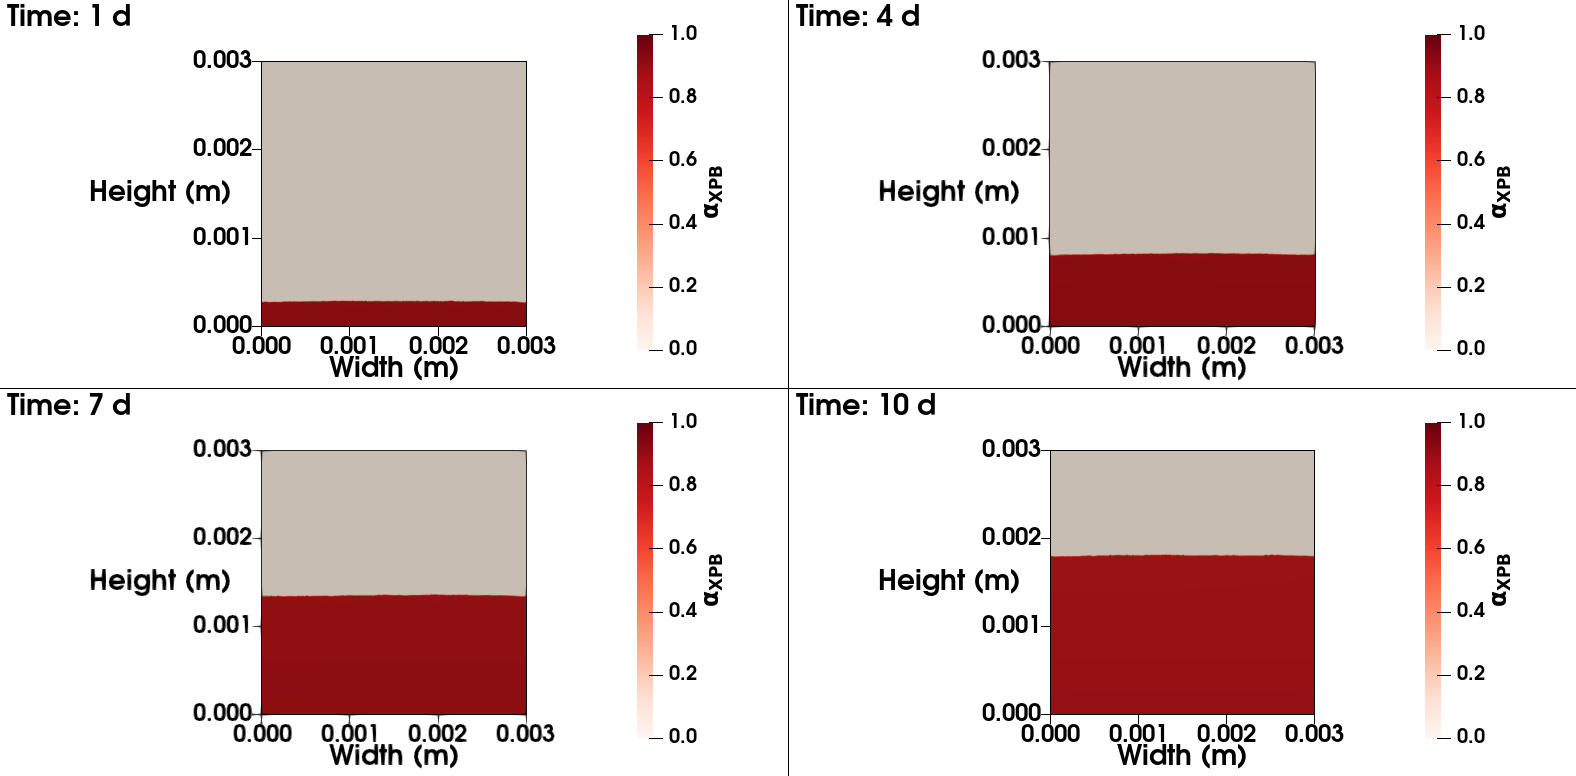
\includegraphics[width=1.1\textwidth,height=0.4\textheight]{Chap4/methods/data/figures/case1_ppb_frac.png}
    \caption{Two dimensional view of PPB as uniformly initiated biofilm over a substratum irradiated at 30 W m\textsuperscript{-2} at 850 nm.} 
    \label{fig:case1_ppb_frac}
\end{figure}

Figure \ref{fig:case1_ppb_frac} shows the growth of PPB biomass at several steps in time. With soluble substrates in excess, PPB grows phototrophically from close to the substratum. New biomass effectively pushes the present biofilm away from the irradiated substratum, with uniformity in the biofilm composition governed by cell motility. In the absence of an external flow field, the biofilm continues to expand without shear stresses controlling any sloughing mechanism. Substrate is still able to be delivered to the highly irradiated regions, however this delivery rate decreases as the biofilm expands. 

\begin{figure}[H]
    \centering
     \hspace*{-1cm}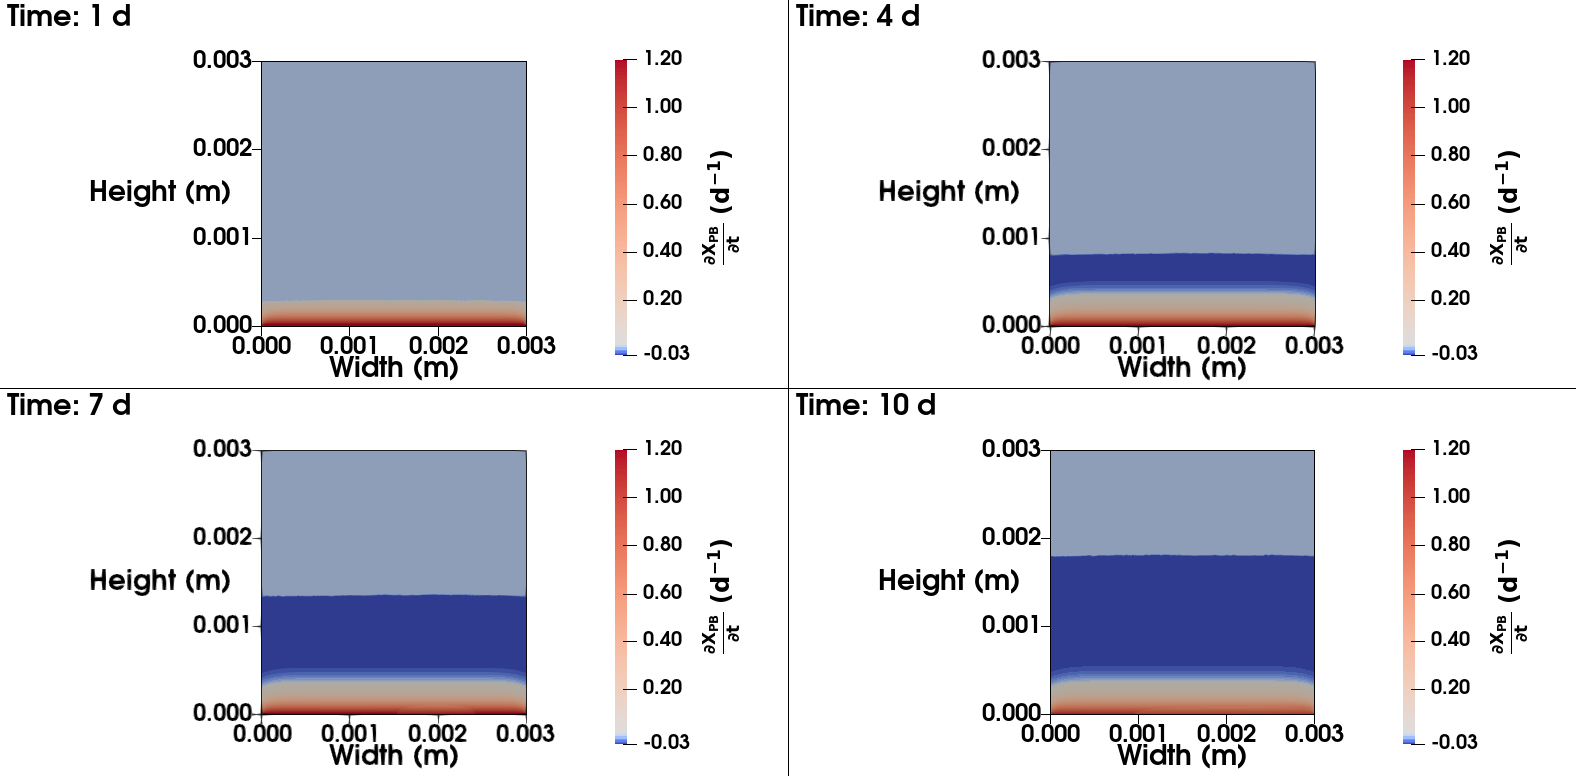
\includegraphics[width=1.1\textwidth,height=0.4\textheight]{Chap4/methods/data/figures/case1_growth_frac.png}
    \caption{Two dimensional view of PPB growth rate as uniformly initiated biofilm over a substratum irradiated at 30 W m\textsuperscript{-2} at 850 nm.} 
    \label{fig:case1_growth_frac}
\end{figure}

Figure \ref{fig:case1_growth_frac} shows the apparent growth rate of PPB over time. There is a 33\% decrease in maximum growth rate over this period as diffusion begins to limit the growth and the initial water volume fraction begins to vacate the biofilm region as particulates start to dominate. Between 4.0 d and the end of the simulation, there is no longer any of the initial pore water in the biofilm domain, so the attenuation of the radiative field cannot explain the reduction in maximum apparent growth rate of PPB. However, the biofilm still includes water in the biofilm void space which doesn't change the apparent diffusivity for a zone of fully developed biofilm. This reduction in growth rate can be attributed to the reduction in delivery of substrate as the solubles need to diffuse through a thicker biofilm to reach the highly irradiated zone of the biofilm.

\begin{figure}[H]
    \centering
    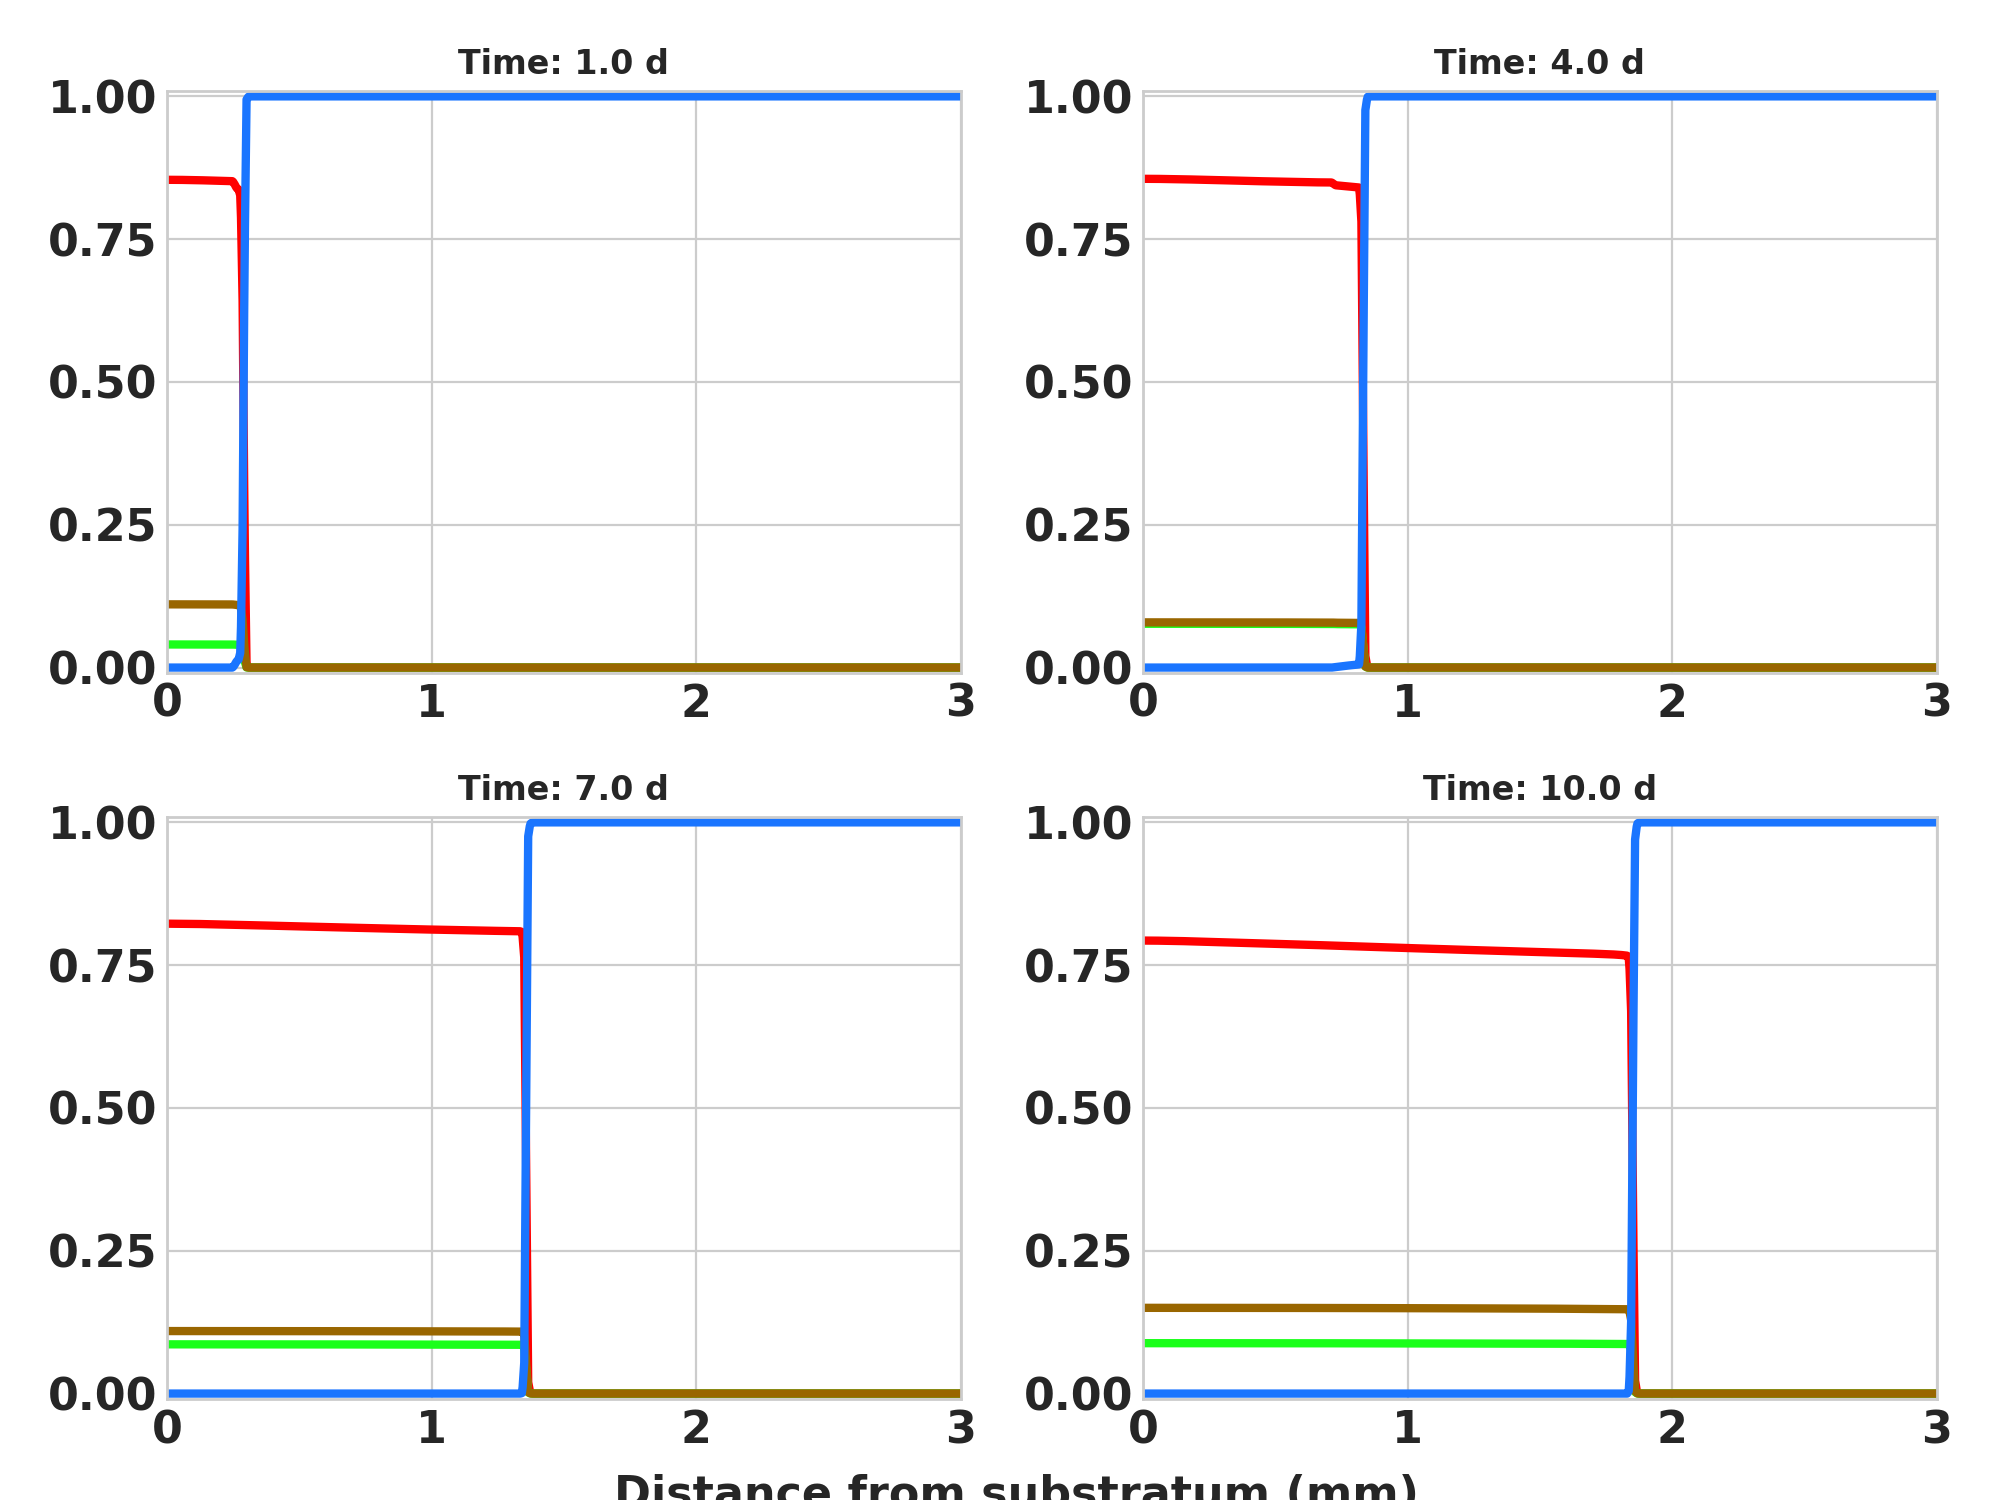
\includegraphics[width=\textwidth,height=0.45\textheight]{Chap4/methods/output/case1.png}
    \caption{Spatial distribution of particulates and water over domain height. Biofilm was initiated as a uniform biofilm over a substratum irradiated at 30 W m\textsuperscript{-2} at 850 nm.} 
    \label{fig:case1_dist_frac}
\end{figure}
 
 Figure \ref{fig:case1_dist_frac} shows the distribution of particulate species along the height of the biofilm. In the absence of other heterotrophic biomass, the spatial distribution of the particulate species has minimal change. As PPB decays, it produces biodegradable particulates, and in turn, inert particulates. Over the period of 10 days, the biofilm front progresses to more than 12 times that of the initial biofilm level. As these cases have not included the shear stresses associated with an externally flowing field, nor the description of a set of detachment rules, the control of the biofilm front has not fully been specified. While this information is not central to this study, it could be included to provide a more complete picture of biofilm evolution in different environments.





\subsection{Case 2: Reduced substratum irradiance}
\begin{figure}[H]
    \centering
     \hspace*{-1cm}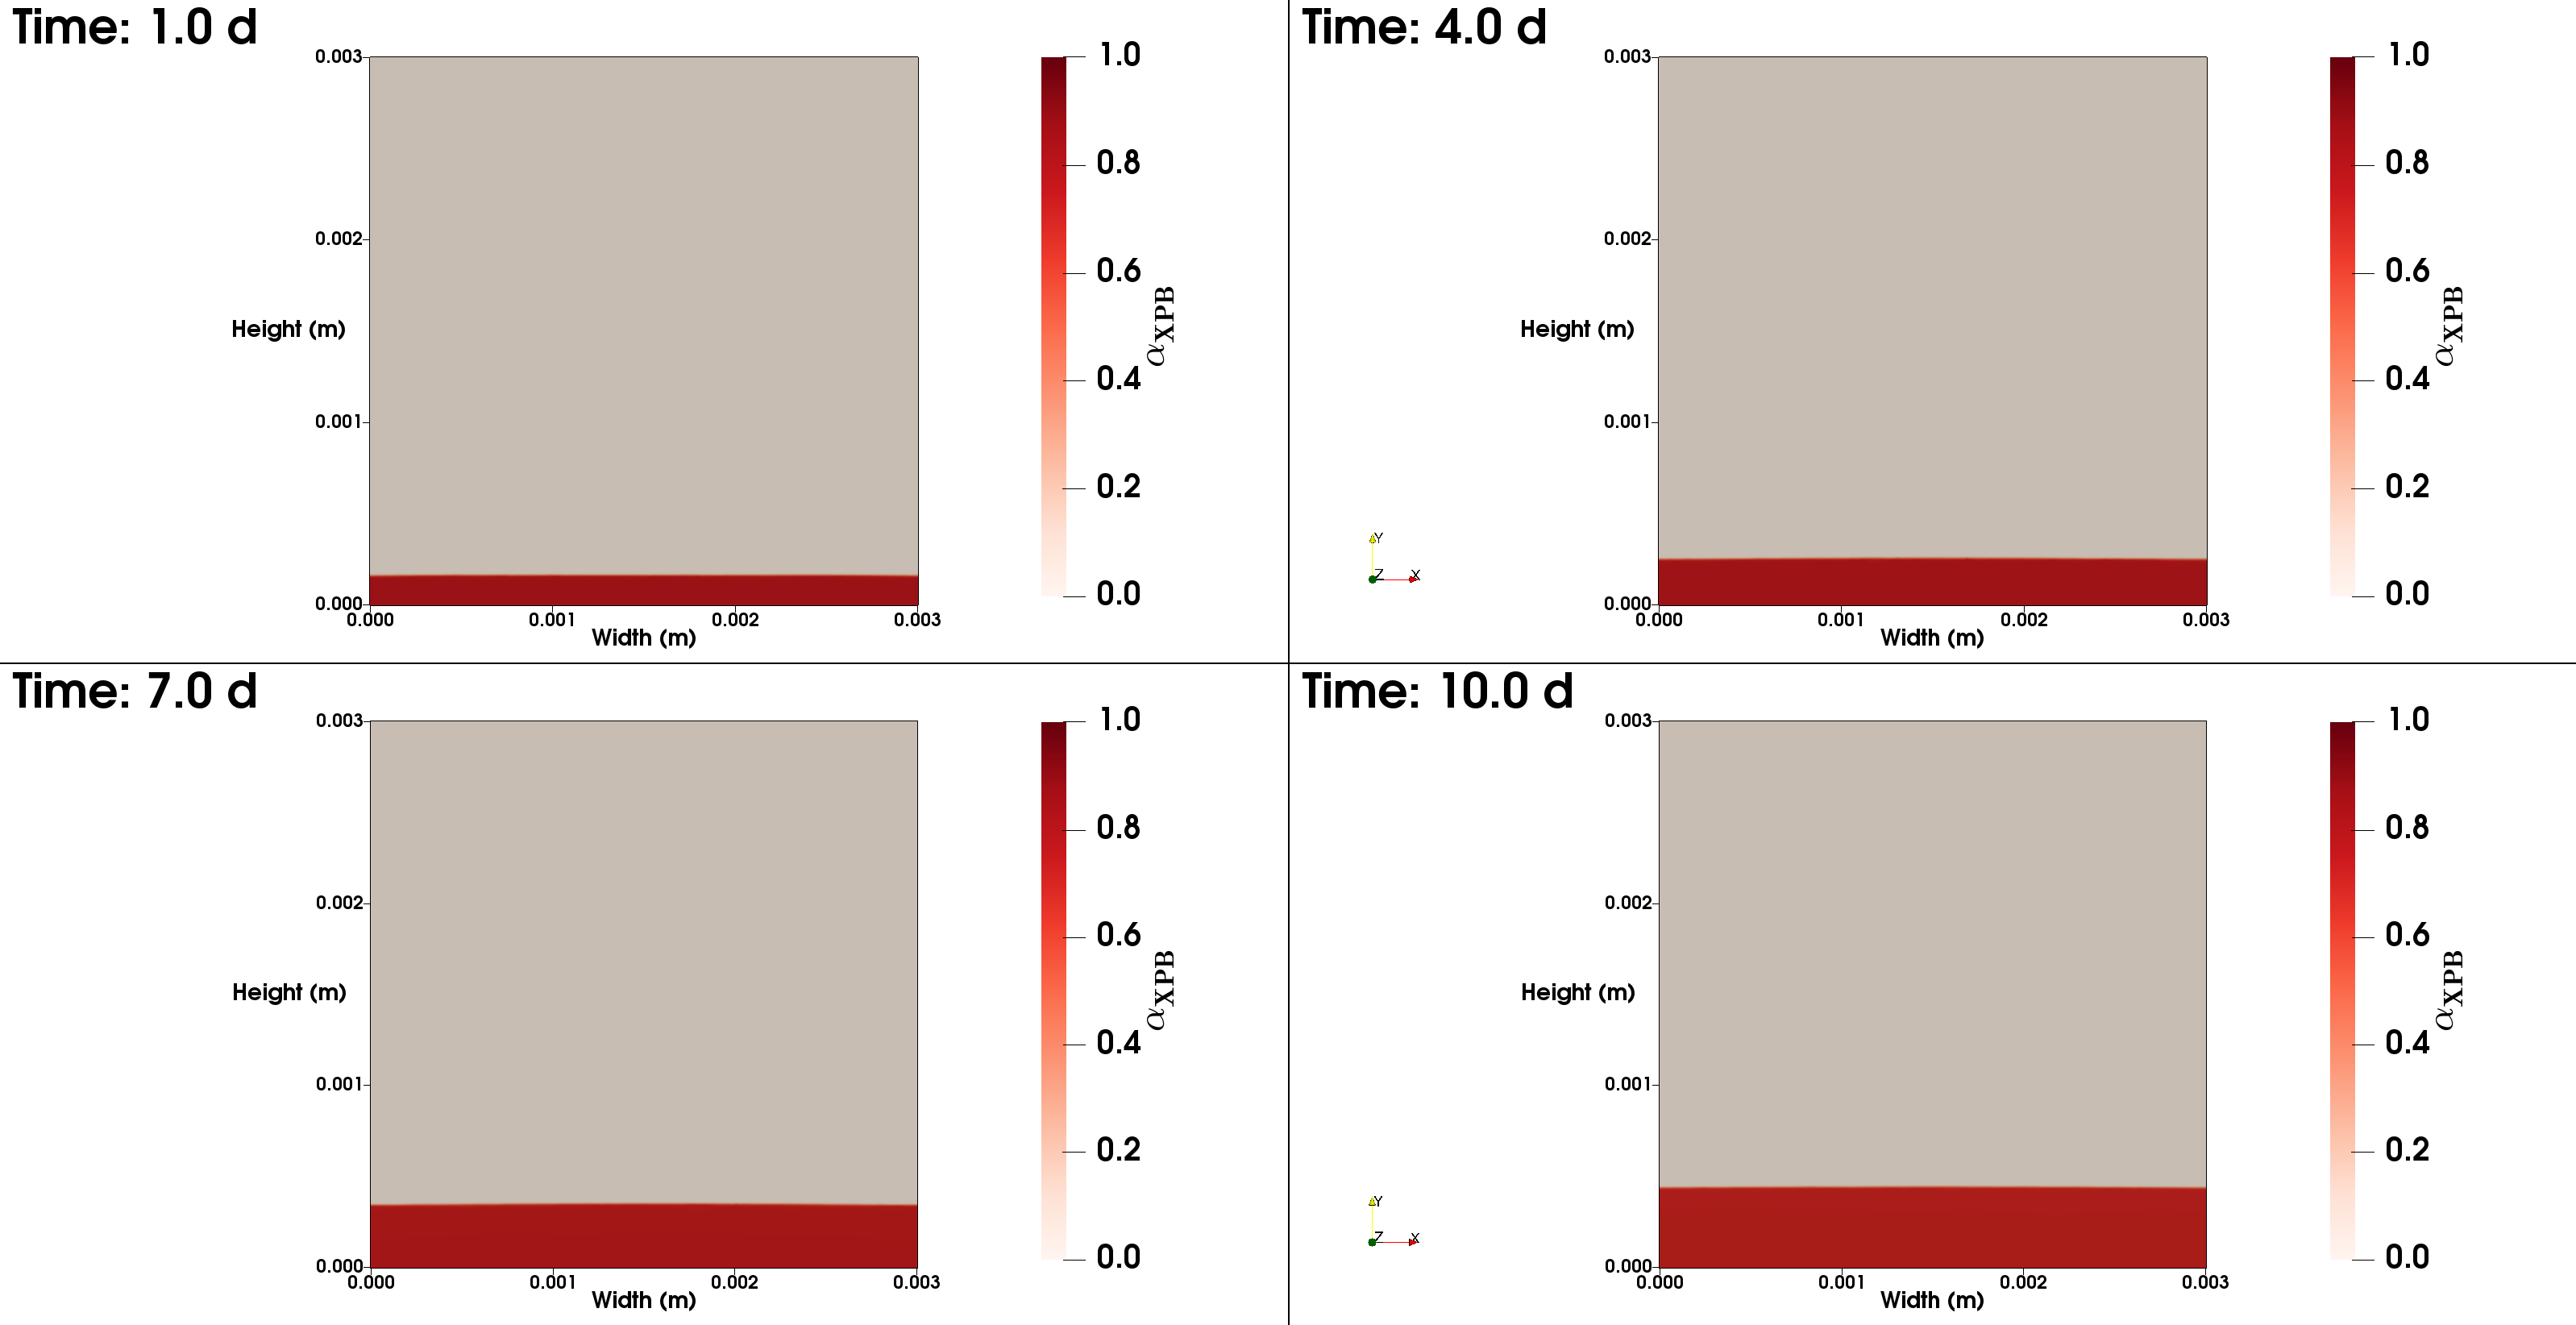
\includegraphics[width=1.1\textwidth,height=0.4\textheight]{Chap4/methods/data/figures/case3_ppb_frac.png}
    \caption{Two dimensional view of PPB as uniformly initiated biofilm over a substratum irradiated at 3 W m\textsuperscript{-2} at 850 nm.} 
    \label{fig:case3_ppb_frac}
\end{figure}

In the case of reduced irradiance from below the biofilm, the absolute growth of biofilm, as well as the apparent growth rate of biofilm are affected. The value of the applied irradiance is 3 W m\textsuperscript{-2} at 850 nm, which is much less than the half-saturation constant of 8.76 W m\textsuperscript{-2} at the same frequency \cite{eltsova2016}. The maximum apparent growth rate is 0.40 d\textsuperscript{-1}. The maximum growth rate stays constant throughout the simulation, most likely due to the low biofilm growth during this time, however we see in the latter stages of the simulation a clear instance of decay, where the irradiance is insufficient to sustain phototrophic activity, and the PPB that initially grew on the substratum begin to decay  as they are pushed further from the radiative field. We see through Fig. \ref{fig:case3_dist_frac} that the biofilm front increases threefold over the 10 day period. The proportion of other particulate matter increases slightly over this time period, and the volume fraction of PPB initially increases from 70\% to 75\%, but then steadies at 70\% as time progresses. 

\begin{figure}[H]
    \centering
     \hspace*{-1cm}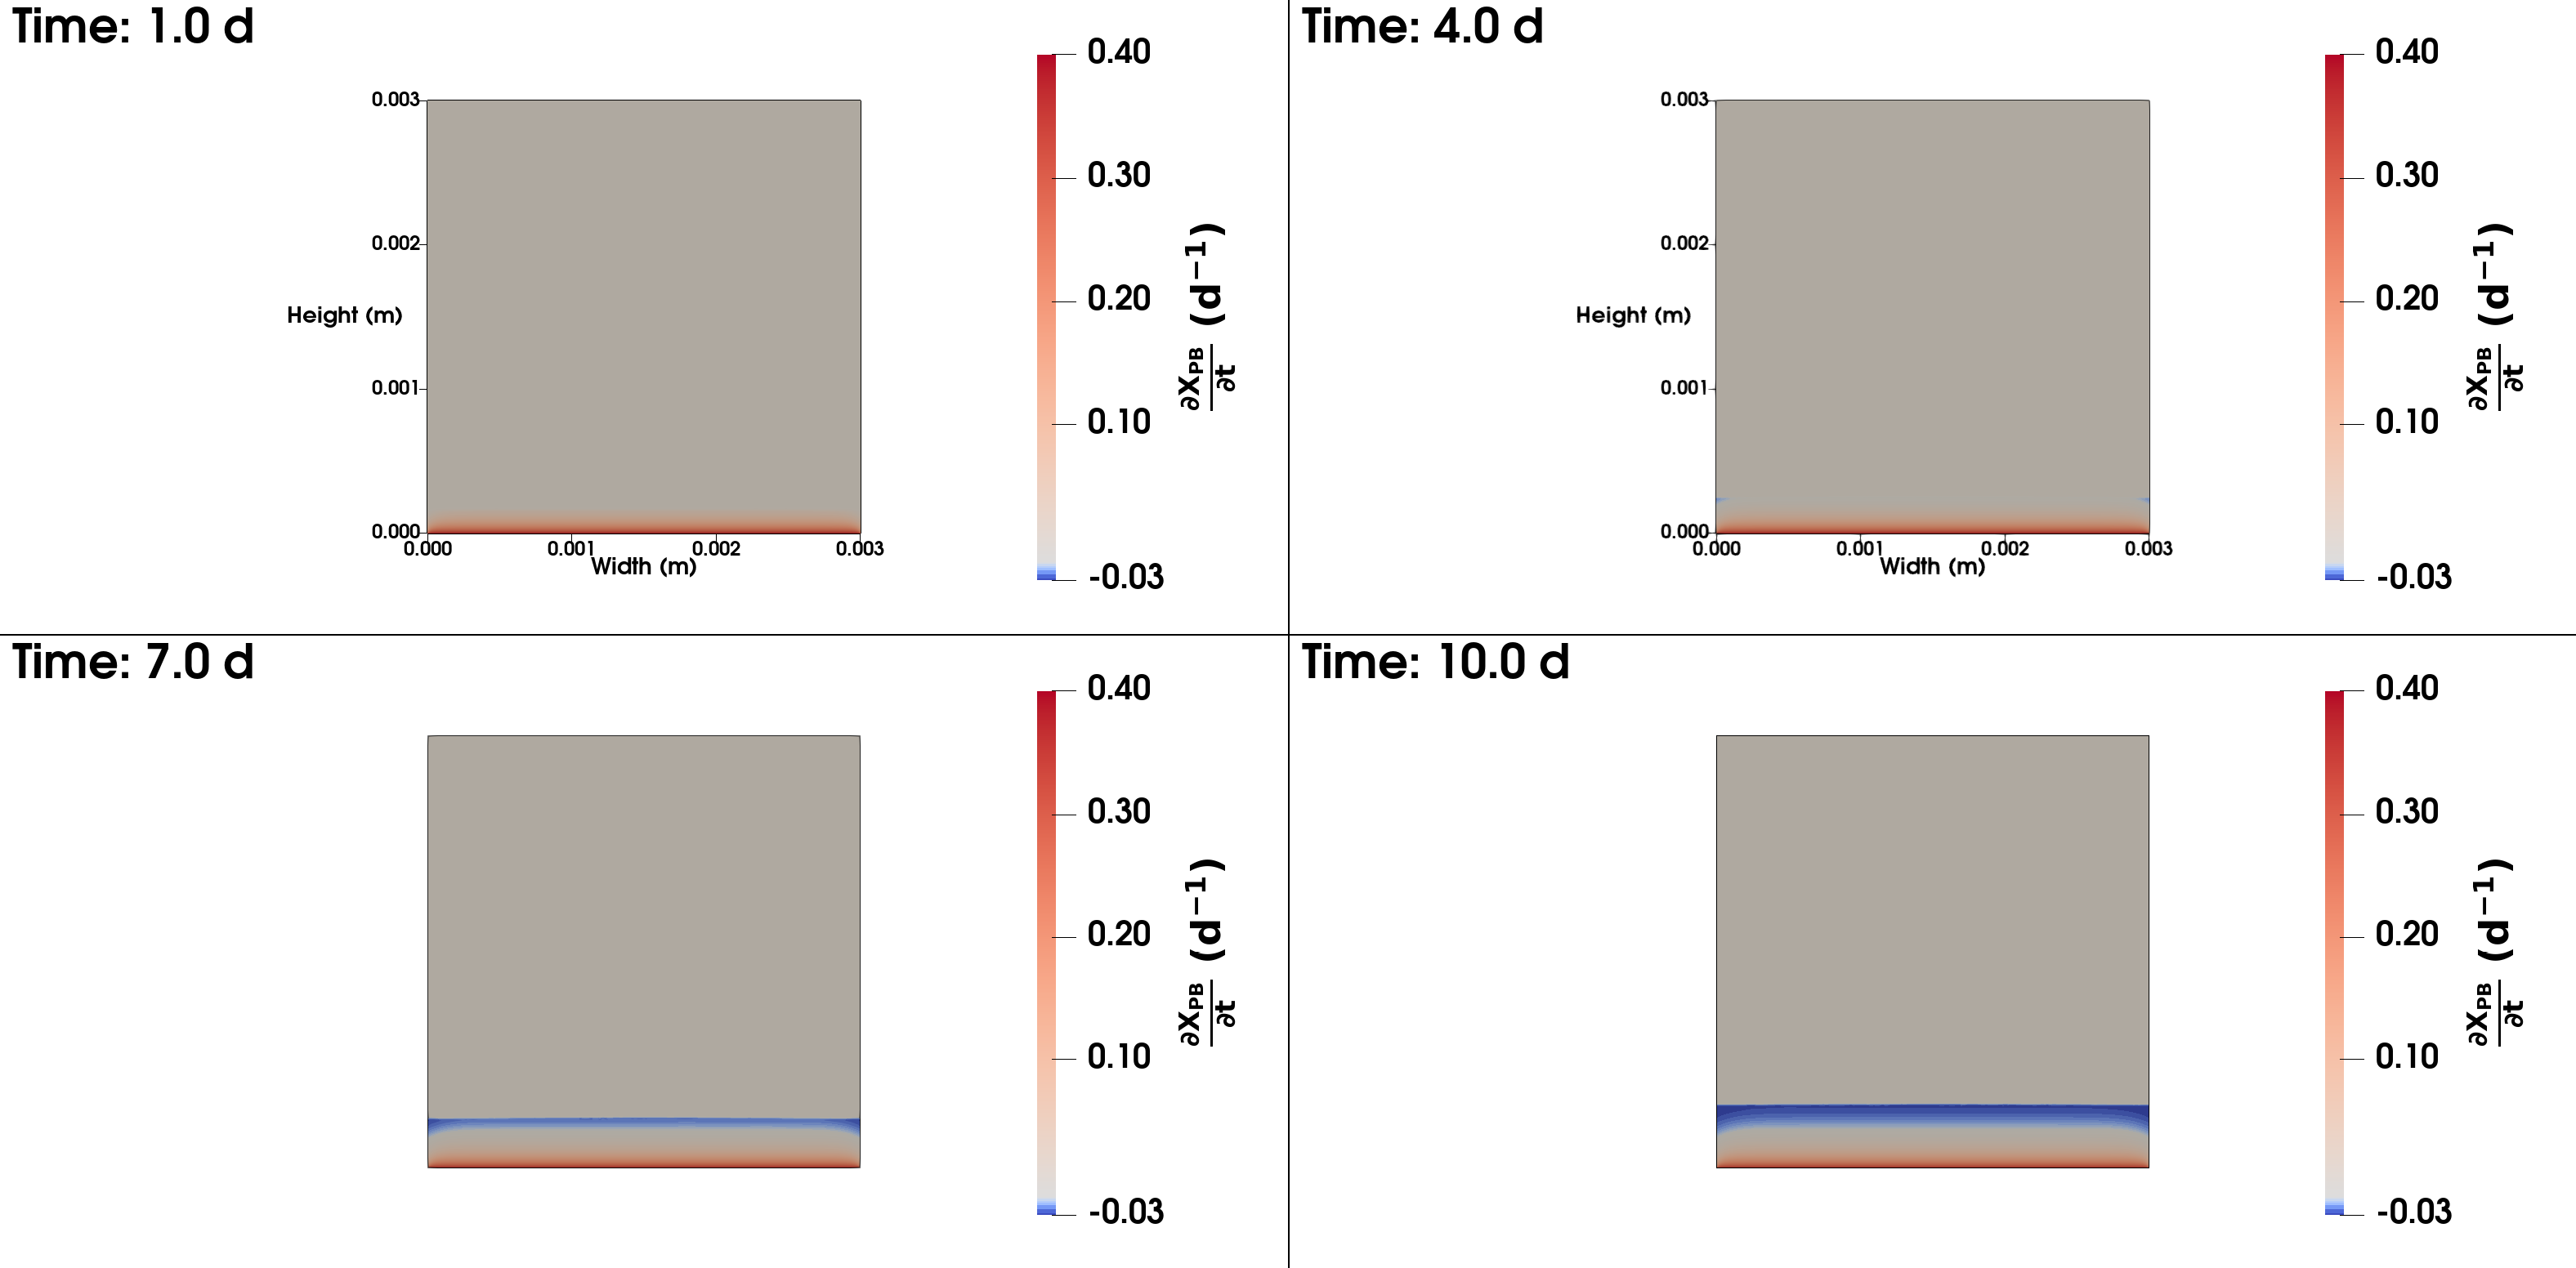
\includegraphics[width=1.1\textwidth,height=0.4\textheight]{Chap4/methods/data/figures/case3_growth_frac.png}
    \caption{Two dimensional view of PPB growth rate as uniformly initiated biofilm over a substratum irradiated at 3 W m\textsuperscript{-2} at 850 nm.} 
    \label{fig:case3_growth_frac}
\end{figure}

\begin{figure}[H]
    \centering
    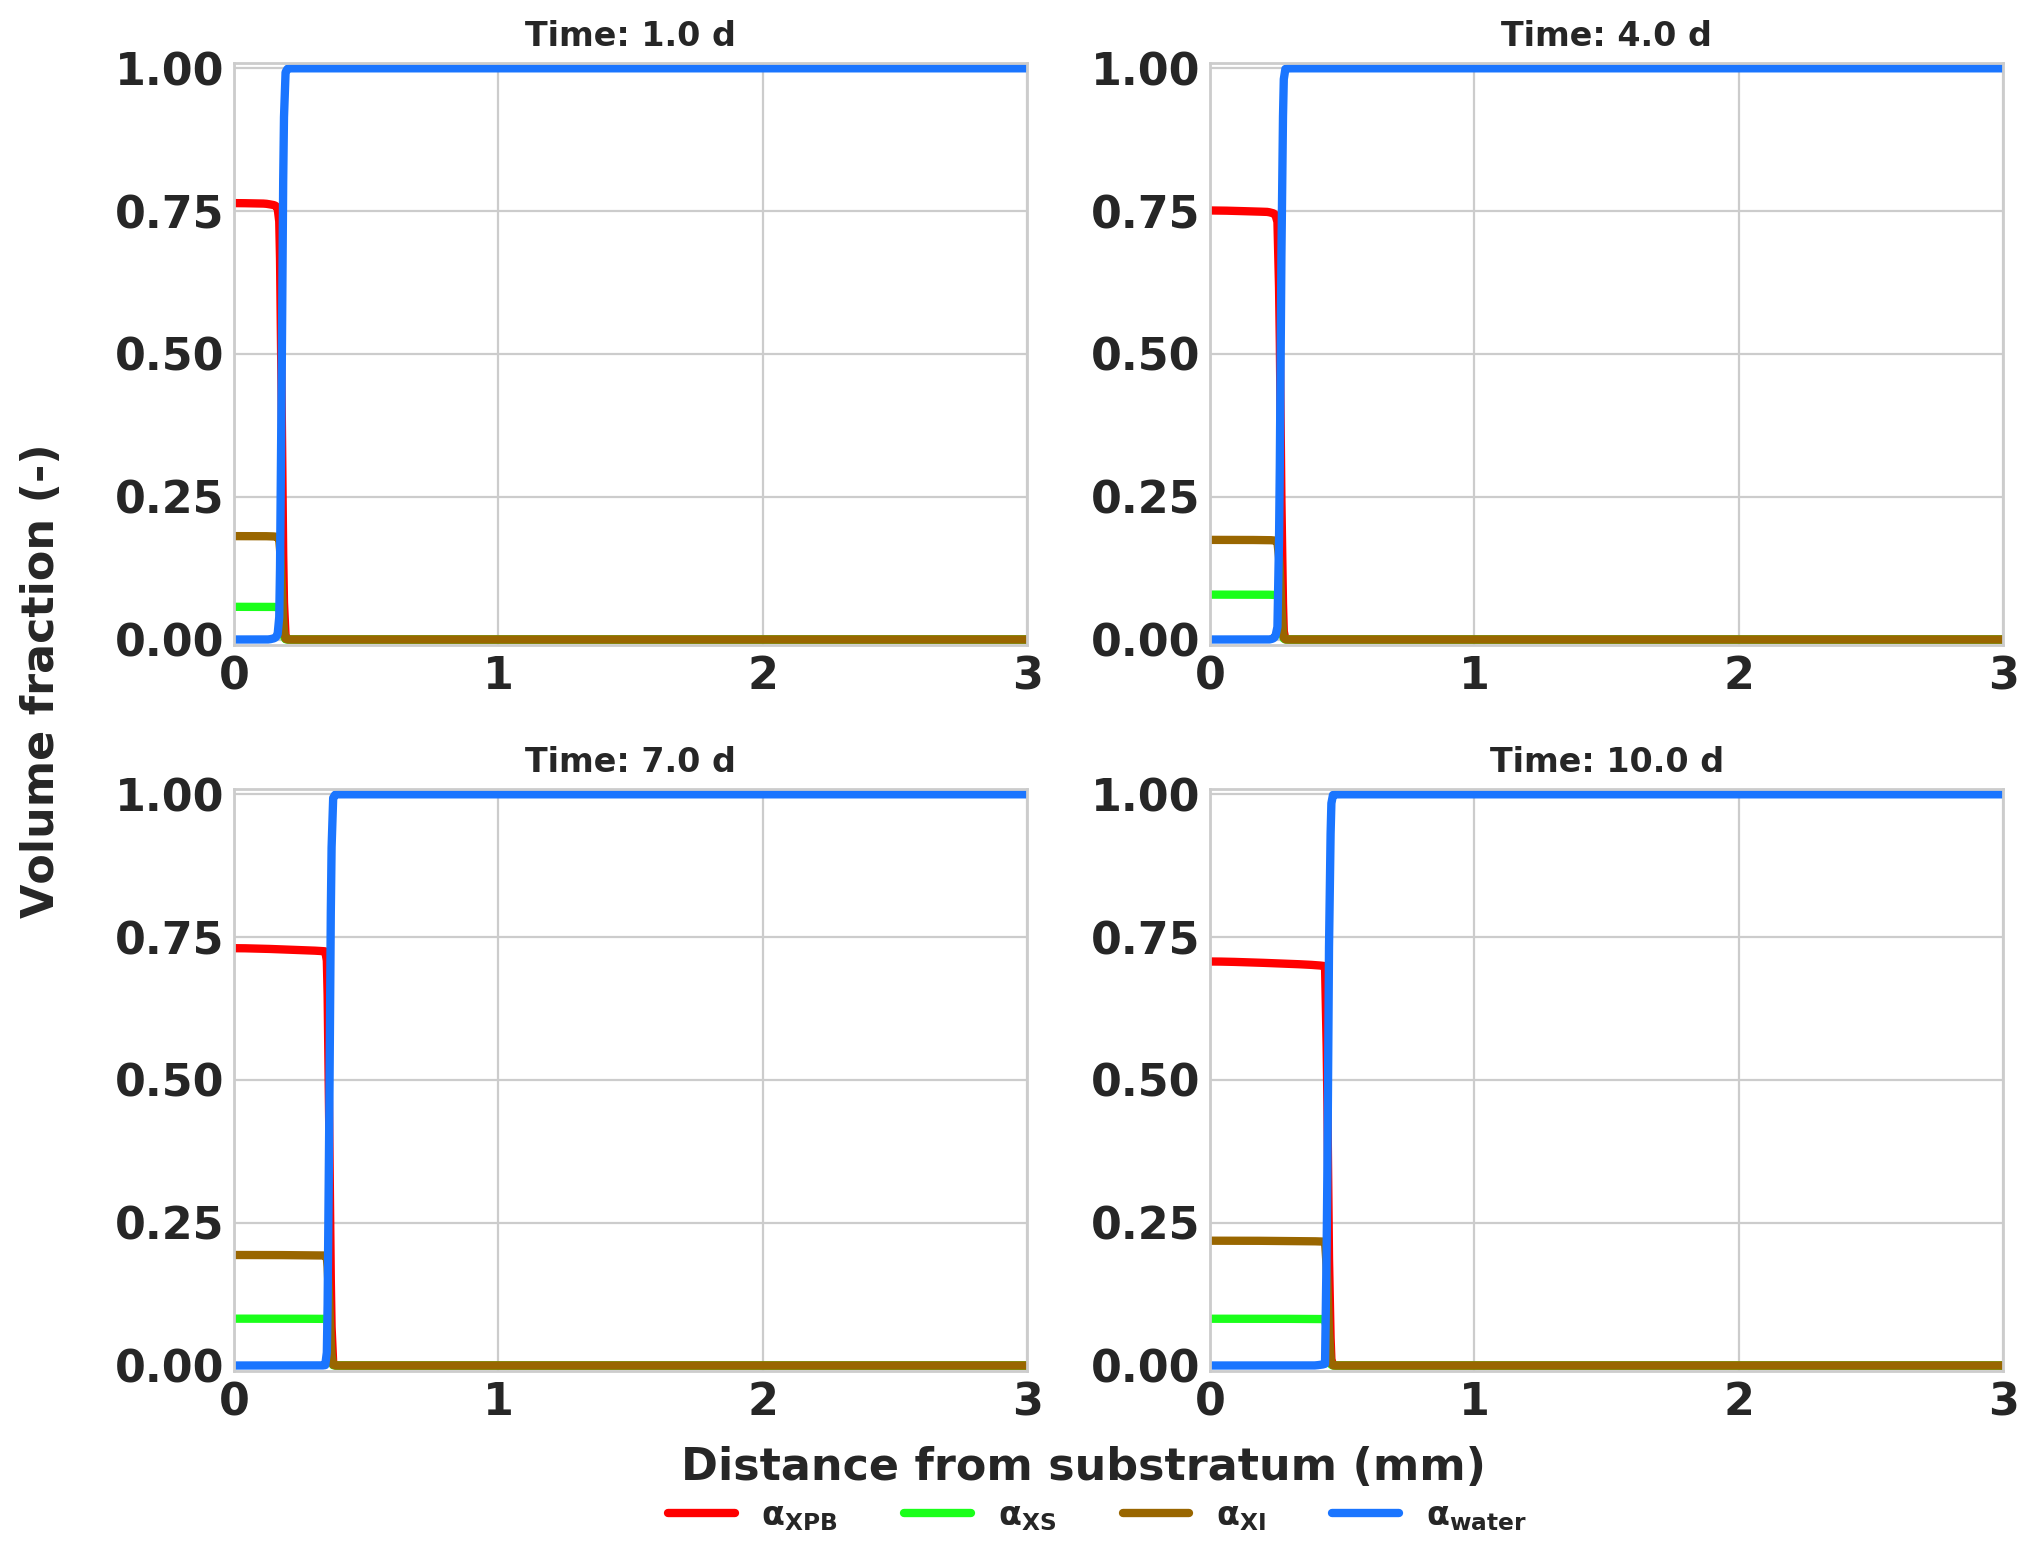
\includegraphics[width=\textwidth,height=0.45\textheight]{Chap4/methods/output/case3.png}
    \caption{Spatial distribution of particulates and water over domain height. Biofilm was initiated as a uniform biofilm over a substratum irradiated at 3 W m\textsuperscript{-2} at 850 nm.} 
    \label{fig:case3_dist_frac}
\end{figure}




\subsection{Case 3: Overhead irradiance}
\begin{figure}[H]
    \centering
     \hspace*{-1cm}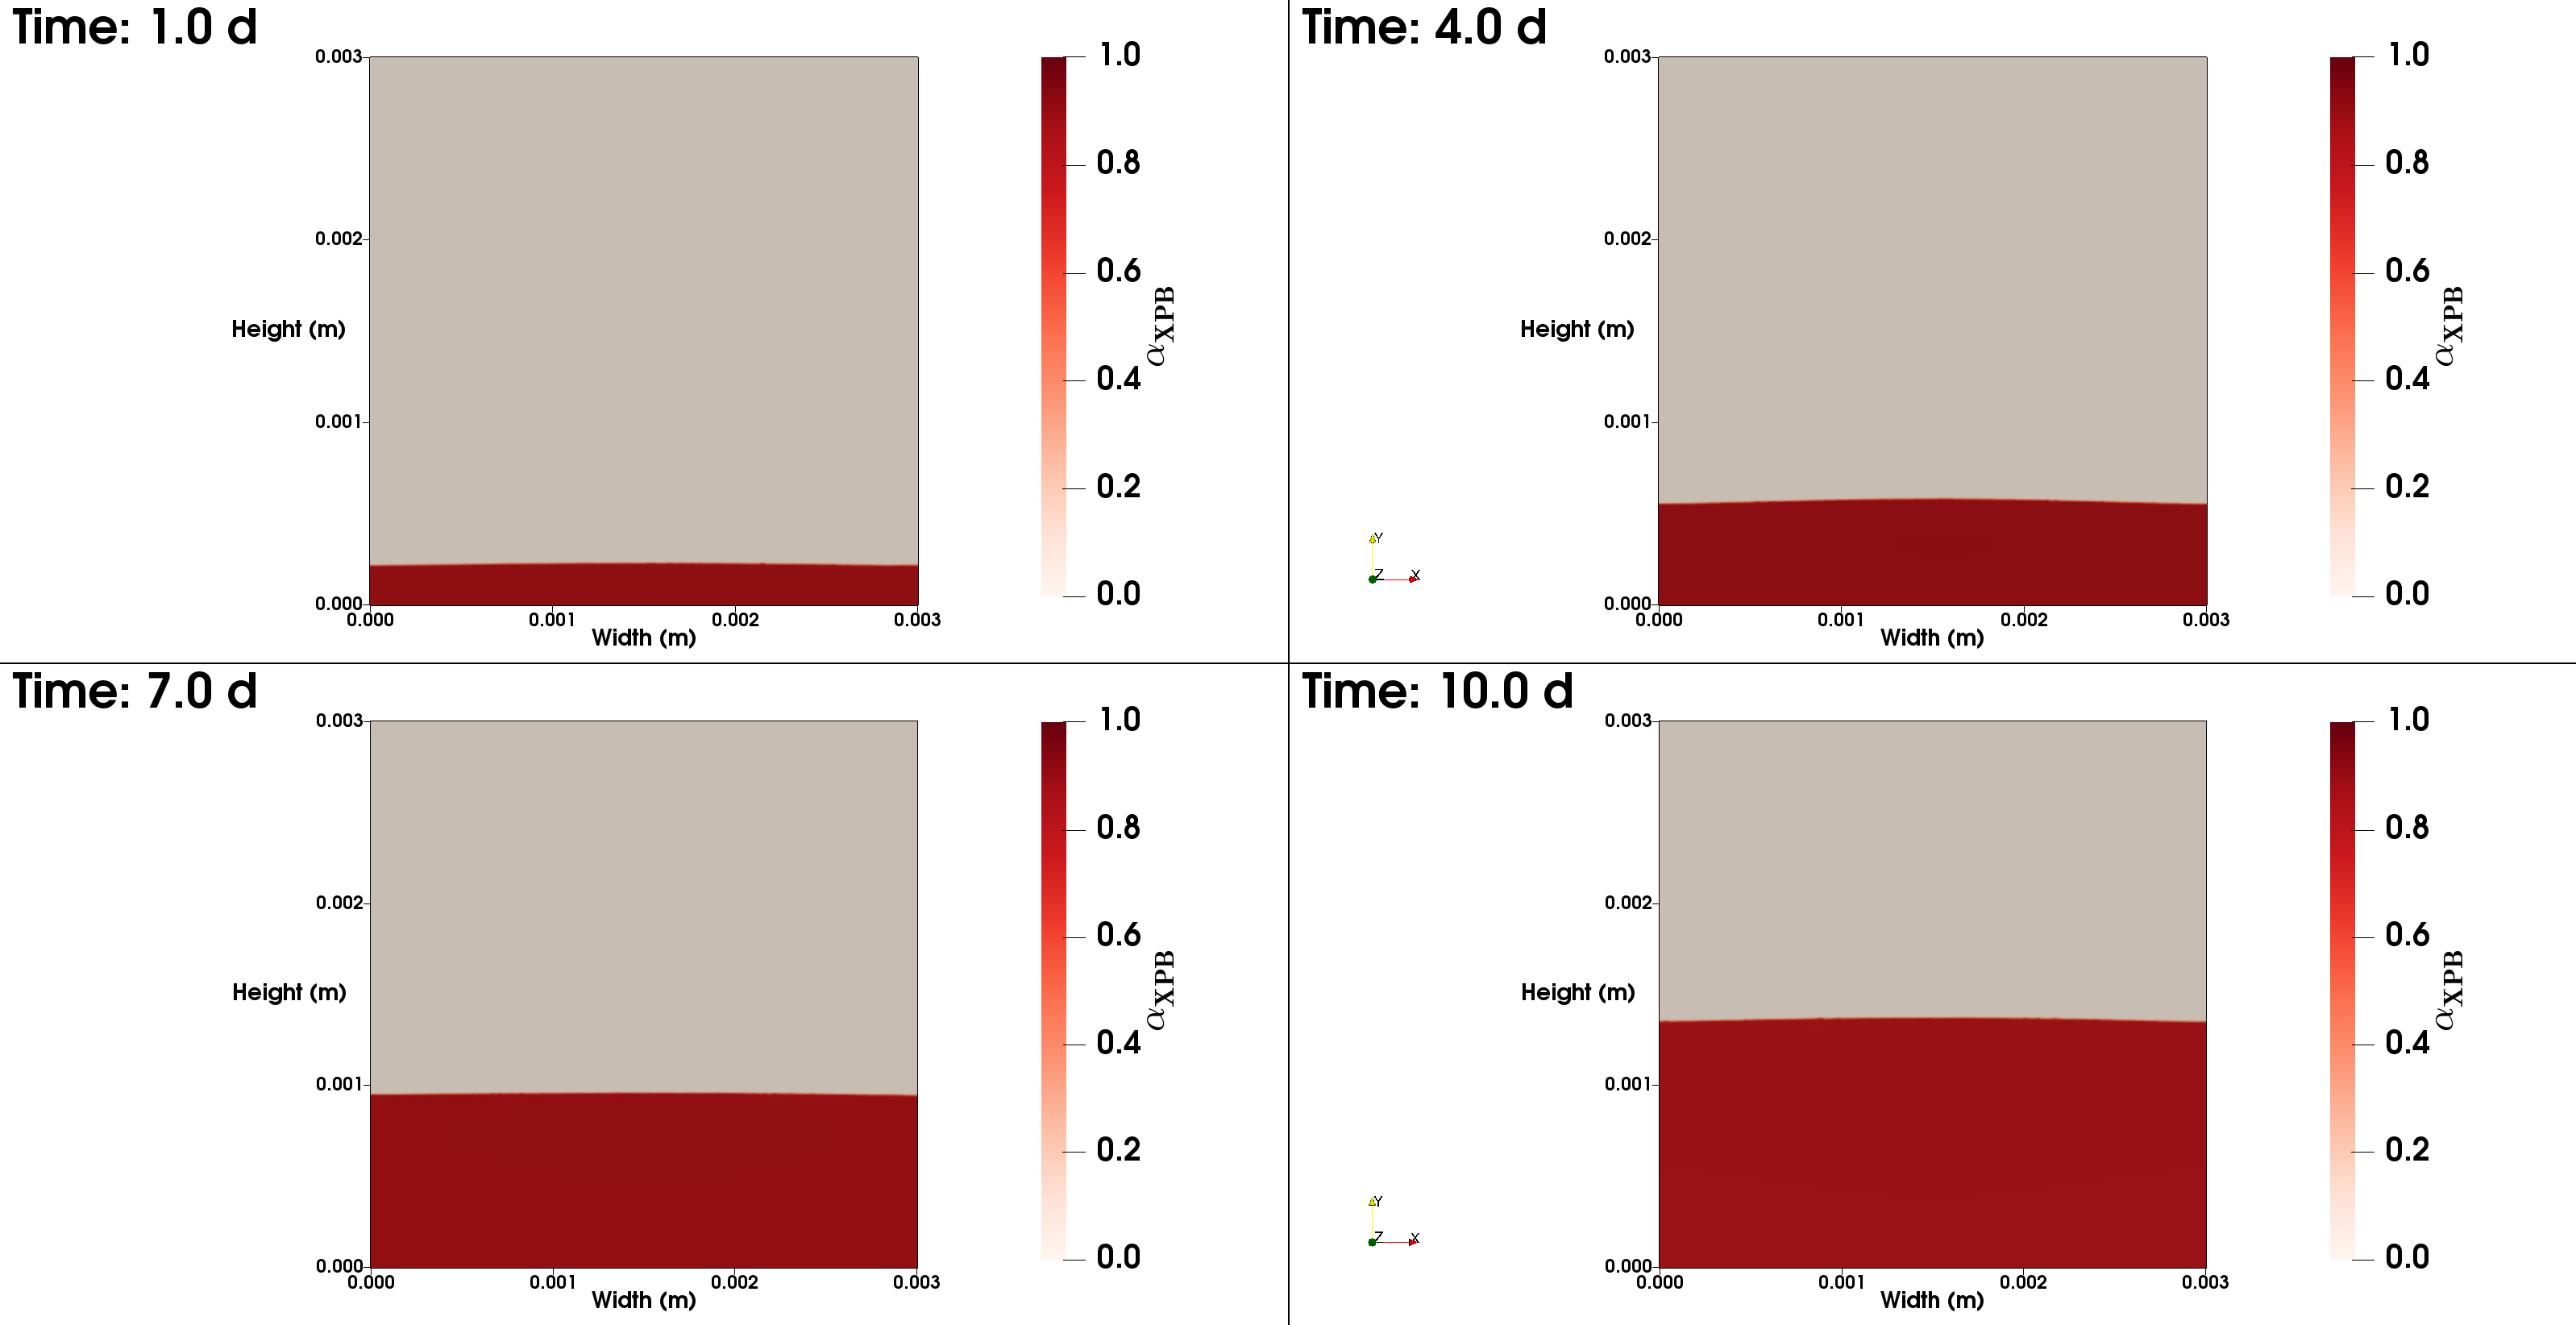
\includegraphics[width=1.1\textwidth,height=0.4\textheight]{Chap4/methods/data/figures/case4_ppb_frac.png}
    \caption{Two dimensional view of PPB as uniformly initiated biofilm irradiated from above at 30 W m\textsuperscript{-2} at 850 nm.} 
    \label{fig:case4_ppb_frac}
\end{figure}

In this simulation, the radiative field was initialised from above the biofilm with an irradiance of 30 W m\textsuperscript{-2}. The biofilm does not reach the same level as that in Case 1, as the radiative field is partly attenuated before it reaches the biofilm. This means that growth is initially steady when compared to Case 1, but it accelerates the the biofilm forms and its front progresses. The initial apparent growth rate is 0.7 d\textsuperscript{-1} and this increases to 1.0 d\textsuperscript{-1} as the biofilm grows. With the in-scattered nature of the radiative field, the intensity is highest at the central point of the boundary. This is due to this point having the most number of neighbours potentially contributing to the radiative field. This results in the biofilm in the early stages of the simulation extending towards this point of highest irradiance. As the simulation progresses and growth is less limited by the irradiance, this biofilm shape becomes less pronounced.

\begin{figure}[H]
    \centering
     \hspace*{-1cm}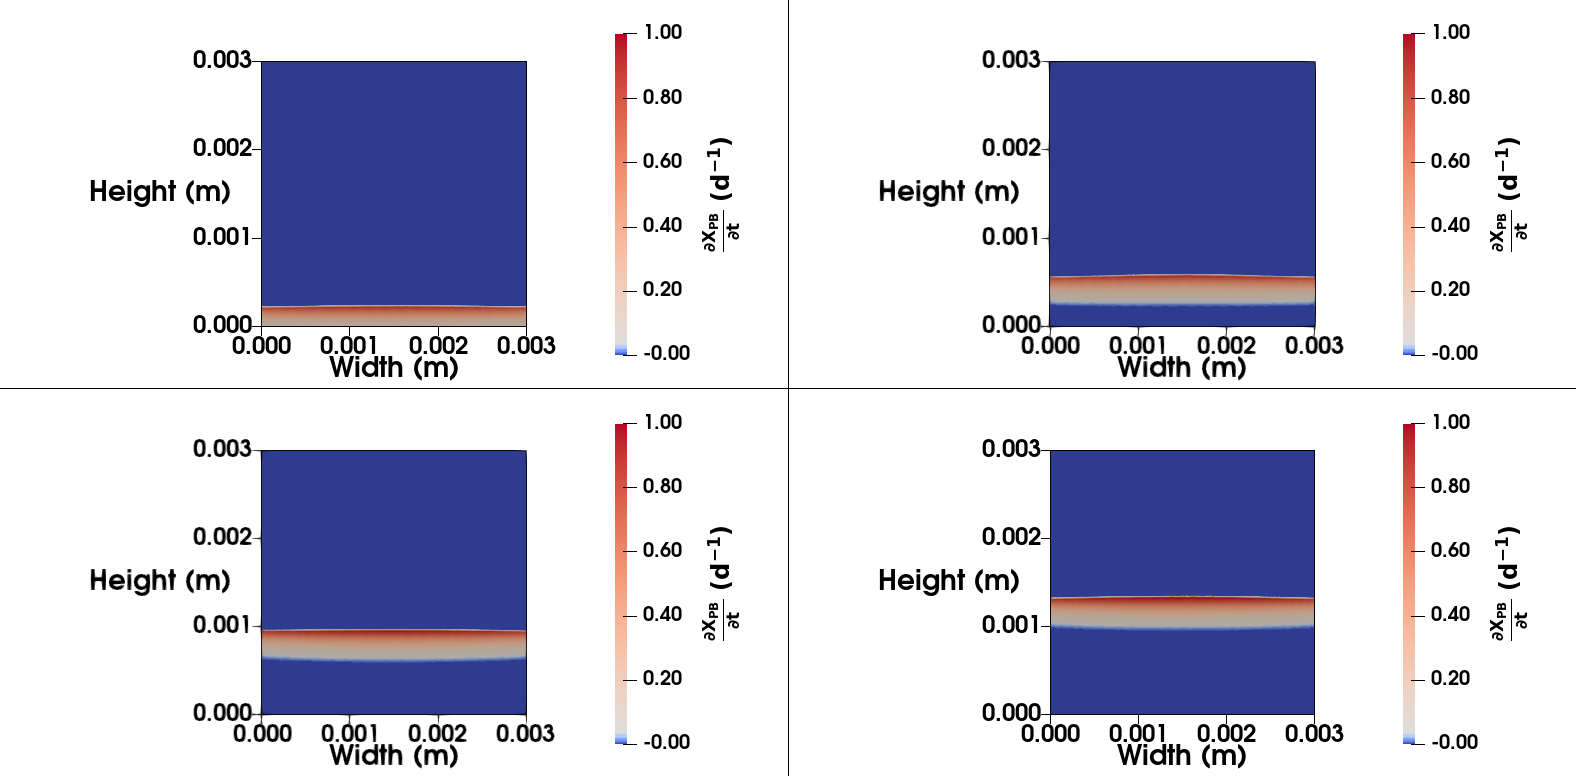
\includegraphics[width=1.1\textwidth,height=0.4\textheight]{Chap4/methods/data/figures/case4_growth_frac.png}
    \caption{Two dimensional view of PPB growth rate as uniformly initiated biofilm irradiated from above at 30 W m\textsuperscript{-2} at 850 nm.} 
    \label{fig:case4_growth_frac}
\end{figure}

\begin{figure}[H]
    \centering
    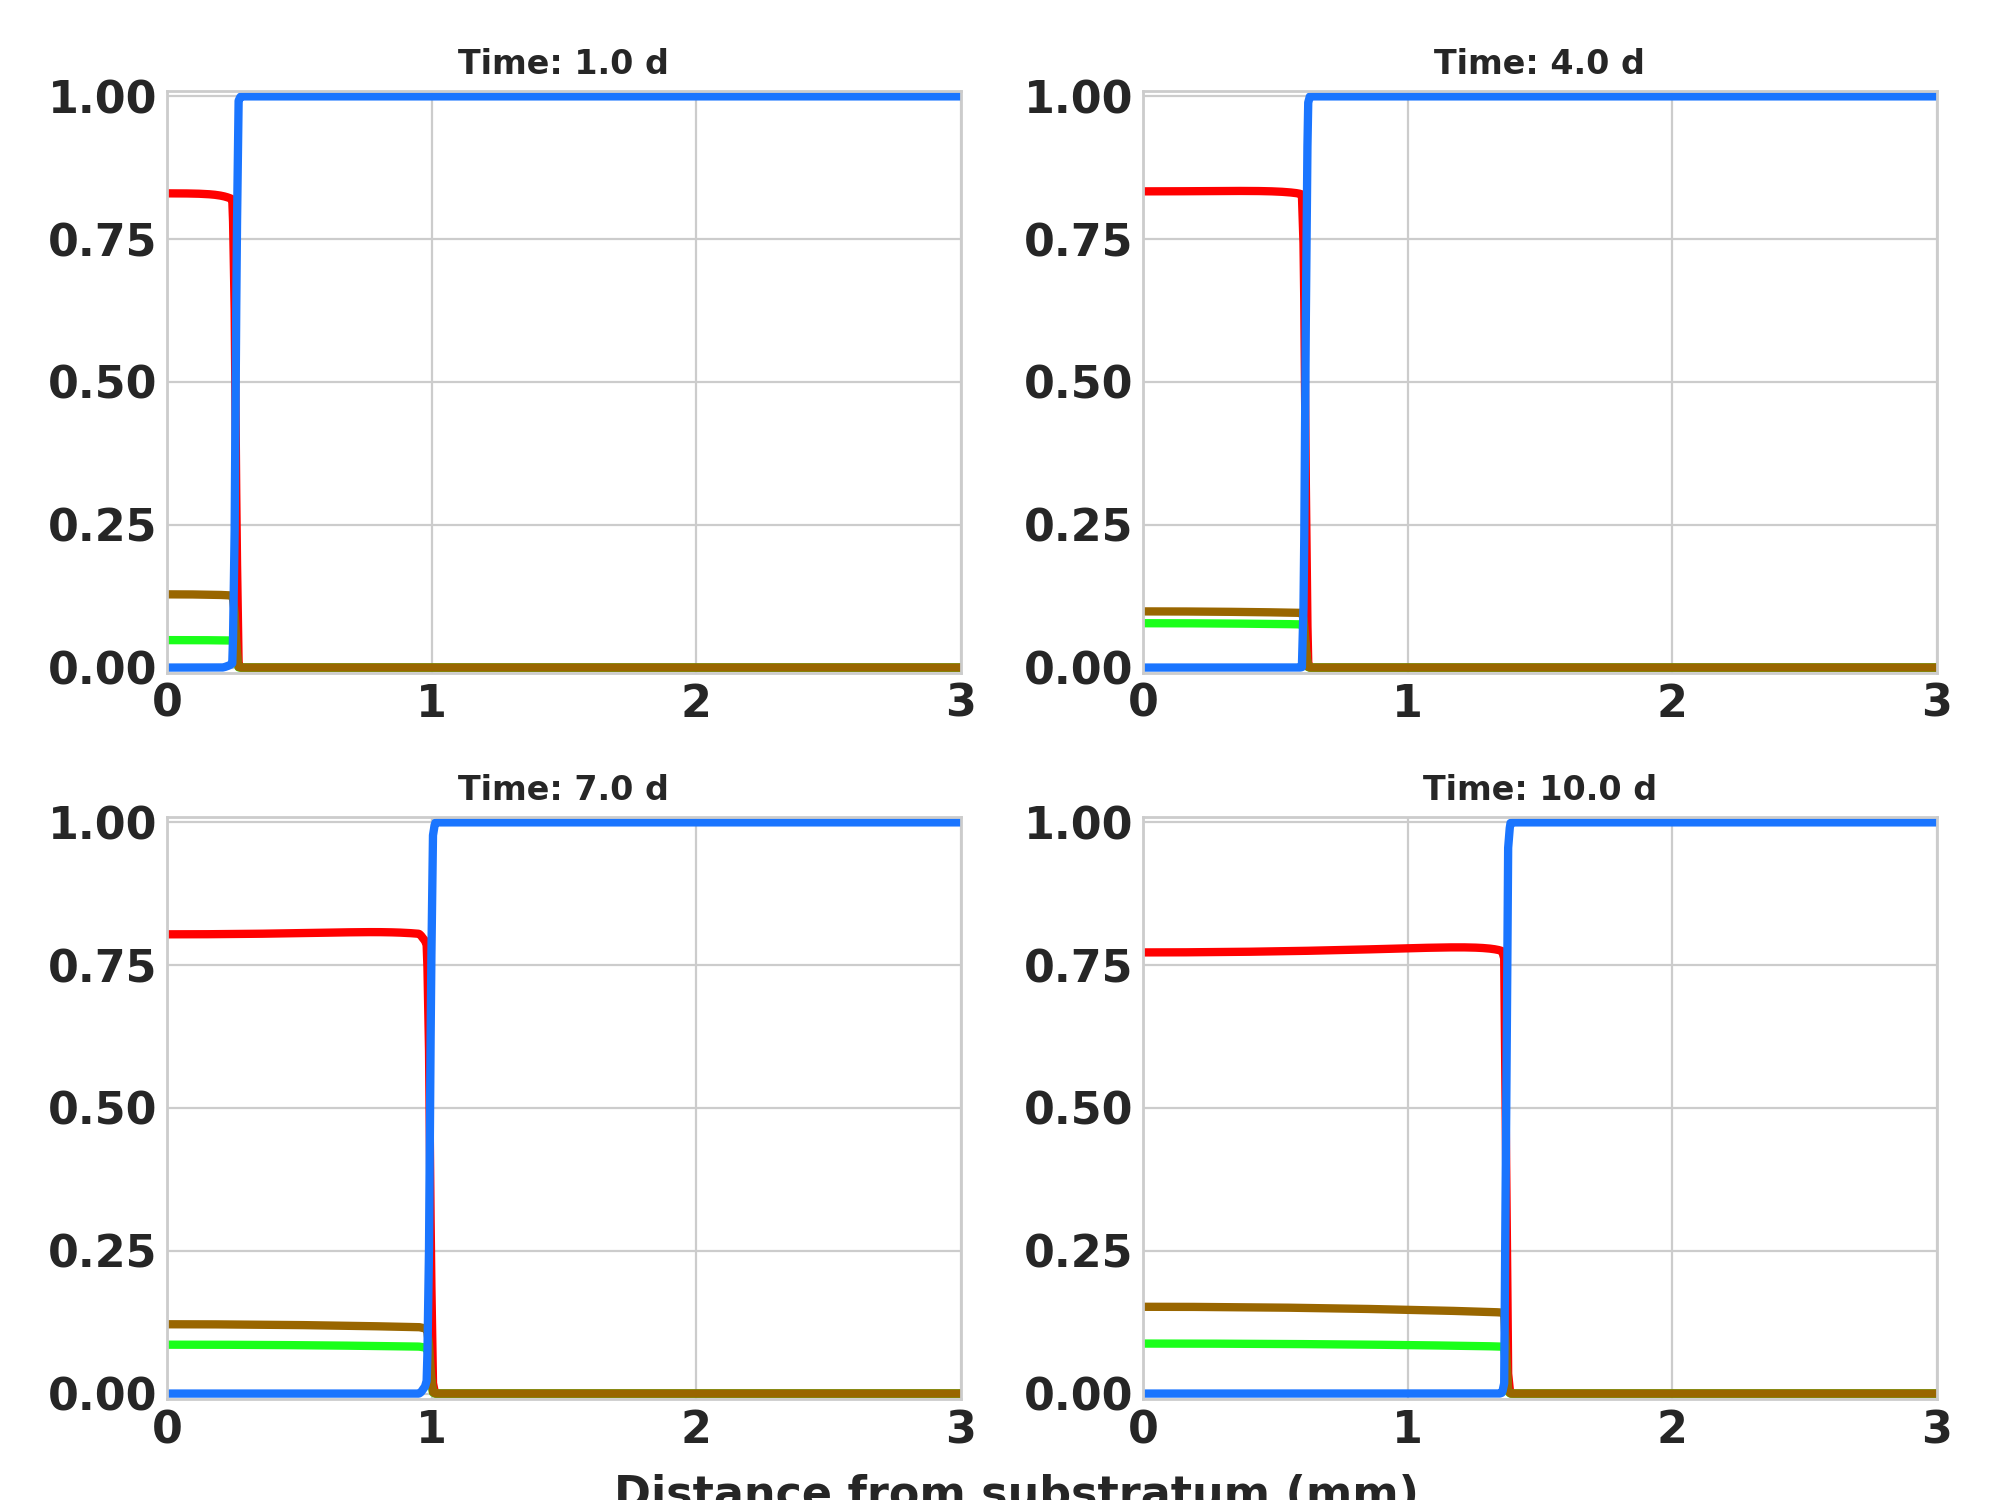
\includegraphics[width=\textwidth,height=0.45\textheight]{Chap4/methods/output/case4.png}
    \caption{Spatial distribution of particulates and water over domain height. Biofilm was initiated as a uniform biofilm irradiated from above at 30 W m\textsuperscript{-2} at 850 nm.} 
    \label{fig:case4_dist_frac}
\end{figure}



\subsection{Case 4: Sparsely initialised biofilm with substratum irradiance}

Figures \ref{fig:case5_ppb_frac}, \ref{fig:case5_growth_frac} and \ref{fig:case5_dist_frac} show the biofilm front in terms of PPB, the distribution of the apparent growth rates for PPB and the spatial distribution of the biofilm components respectively. The system is initialised with 3 hemispherical (or cylindrical in 2 dimensions) zones of biofilm along the substratum. The two partial  spheres initialised in the corners begin at the origin and have a radius of 0.18 mm. The partial sphere initialised in the centre of the horizontal axis has a radius of 0.25 mm. 

\begin{figure}[H]
    \centering
     \hspace*{-1cm}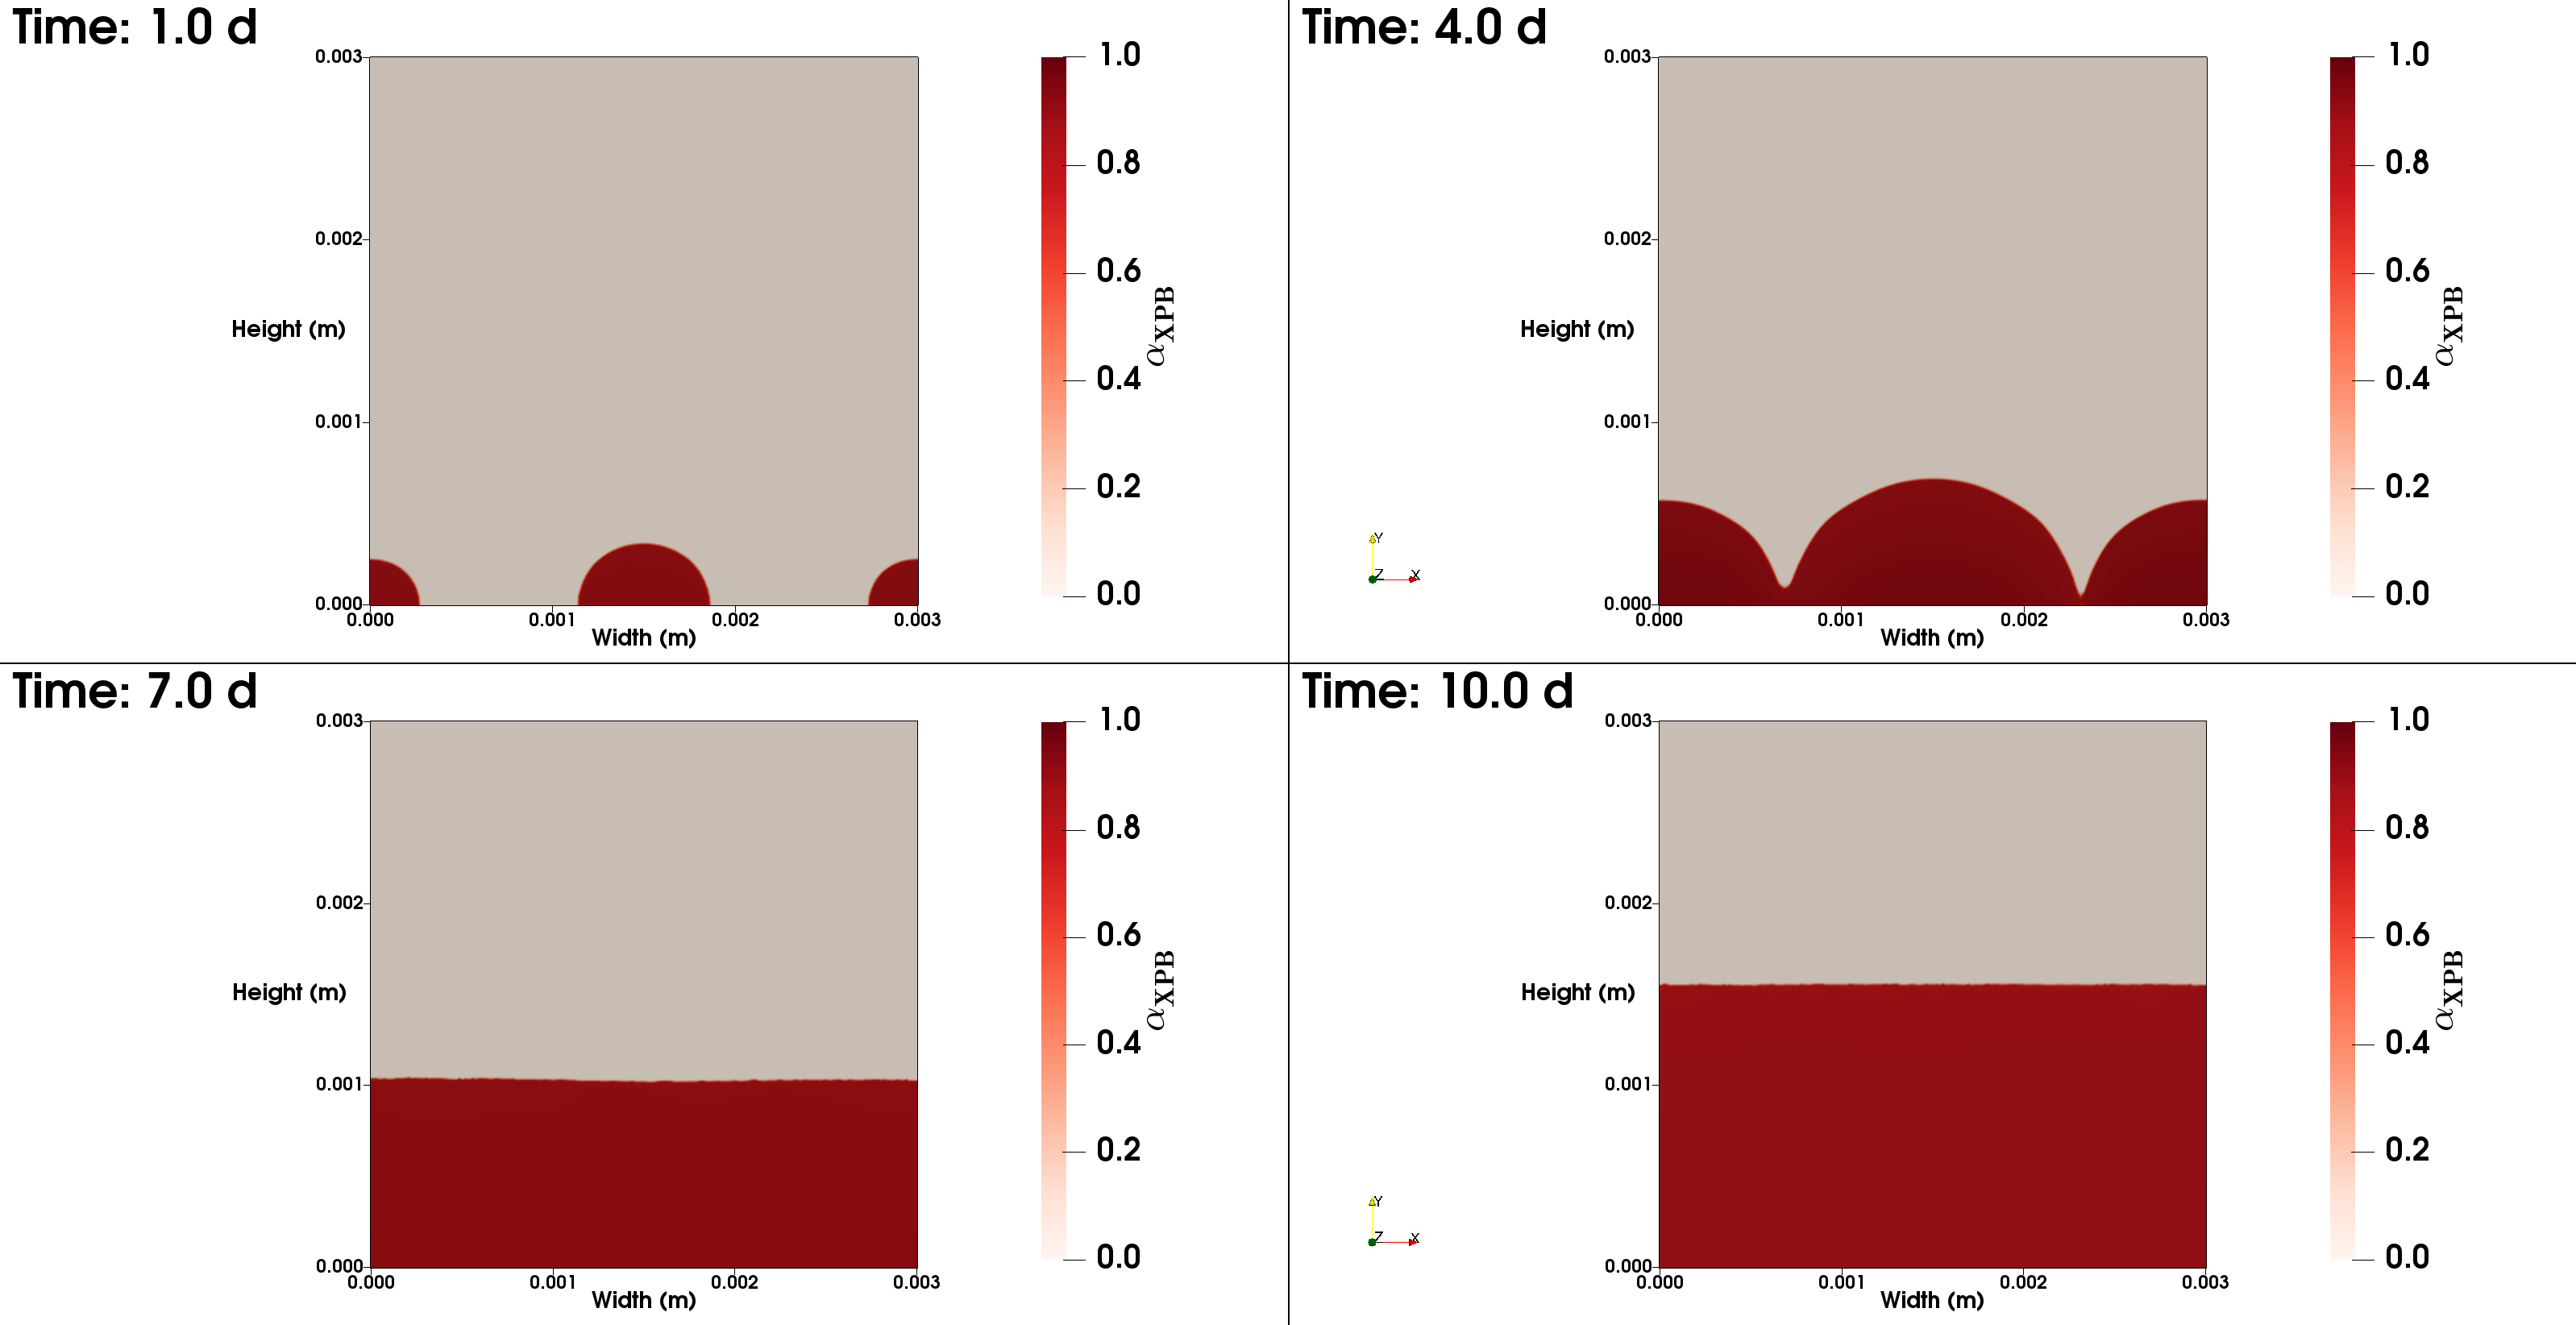
\includegraphics[width=1.1\textwidth,height=0.4\textheight]{Chap4/methods/data/figures/case5_ppb_frac.png}
    \caption{Two dimensional view of PPB as sparsely initiated biofilm over a substratum irradiated at 30 W m\textsuperscript{-2} at 850 nm.} 
    \label{fig:case5_ppb_frac}
\end{figure}

Figure \ref{fig:case5_ppb_frac} depicts the biofilm structure as growth occurs over the 10 day period. With the radiative field being deployed from below the substratum, new biomass occupies the space in the region close to this field. Older biomass is pushed away from the substratum where the apparent growth rate tends to the decay rate. 

\begin{figure}[H]
    \centering
    \hspace*{-1cm}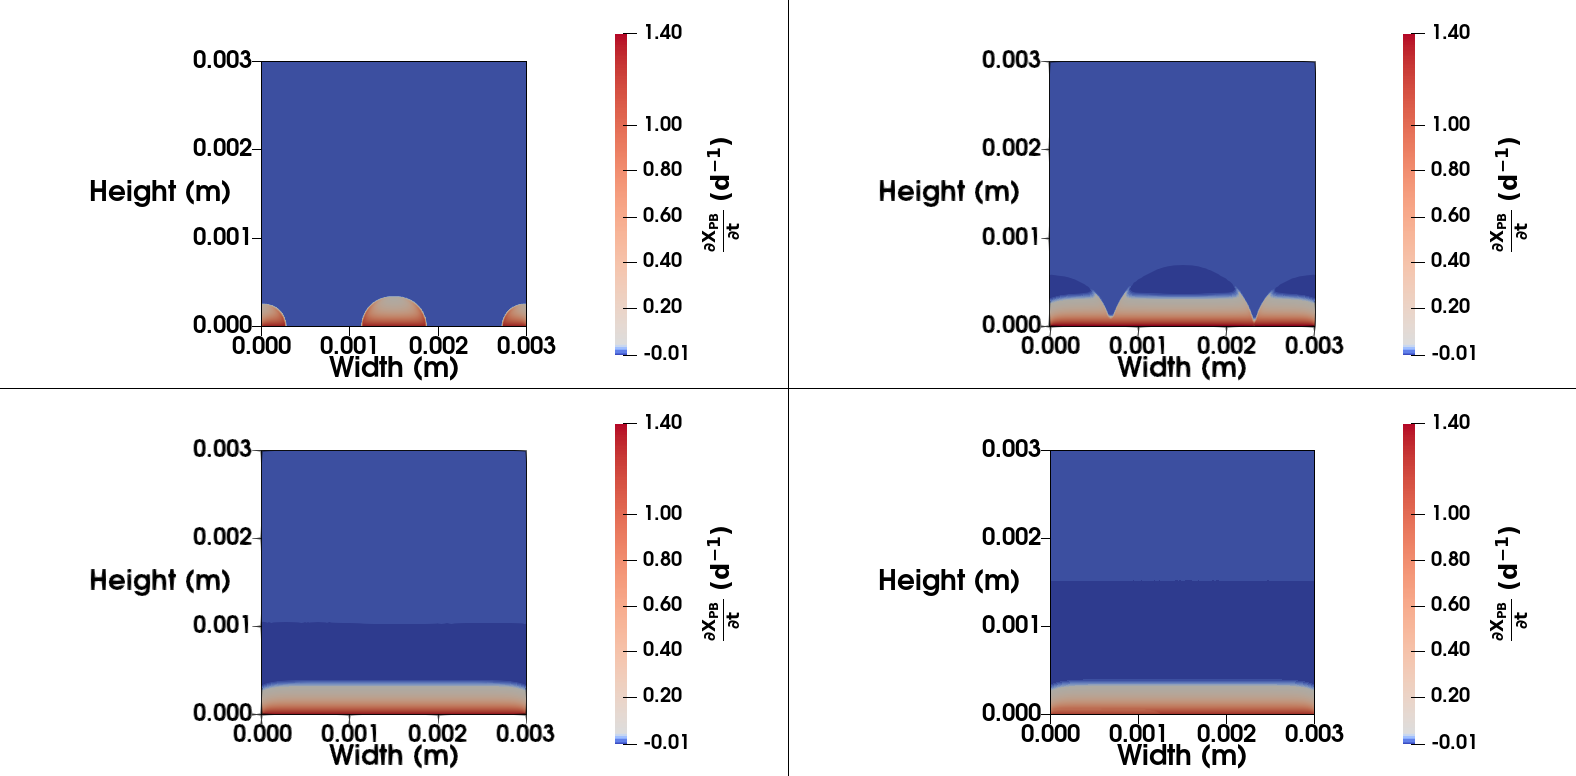
\includegraphics[width=1.1\textwidth,height=0.4\textheight]{Chap4/methods/data/figures/case5_growth_frac.png}
    \caption{Two dimensional view of PPB growth rate as sparsely initiated biofilm over a substratum irradiated at 30 W m\textsuperscript{-2} at 850 nm.} 
    \label{fig:case5_growth_frac}
\end{figure}

Figure \ref{fig:case5_growth_frac} demonstrates the growth of PPB, which effectively follows the intensity of the radiative field. The maximum apparent growth rate is constant at 1.4 d\textsuperscript{-1}. As the biofilm grows, the apparent growth rate diminishes, tending slightly negative where the radiative field is insufficient for phototrophic growth, or to zero for regions where there is no biomass in the domain. The apparent growth rate only becomes slightly negative in the region away from the substratum. The difference in attenuation coefficients (the sum of scattering and absorption coefficients) between the water phase and the biofilm phase is clearly demonstrated in the Fig. \ref{fig:case5_growth_frac} at 4.0 d, where the radiative field is less attenuated through water than through the biofilm, and this results in the edges of the biofilm having a greater growth rate than the interior. This phenomenon is even more pronounced in Fig. \ref{fig:case6_growth_frac} where the radiative field is initialised from above the biofilm. 

\begin{figure}[H]
    \centering
    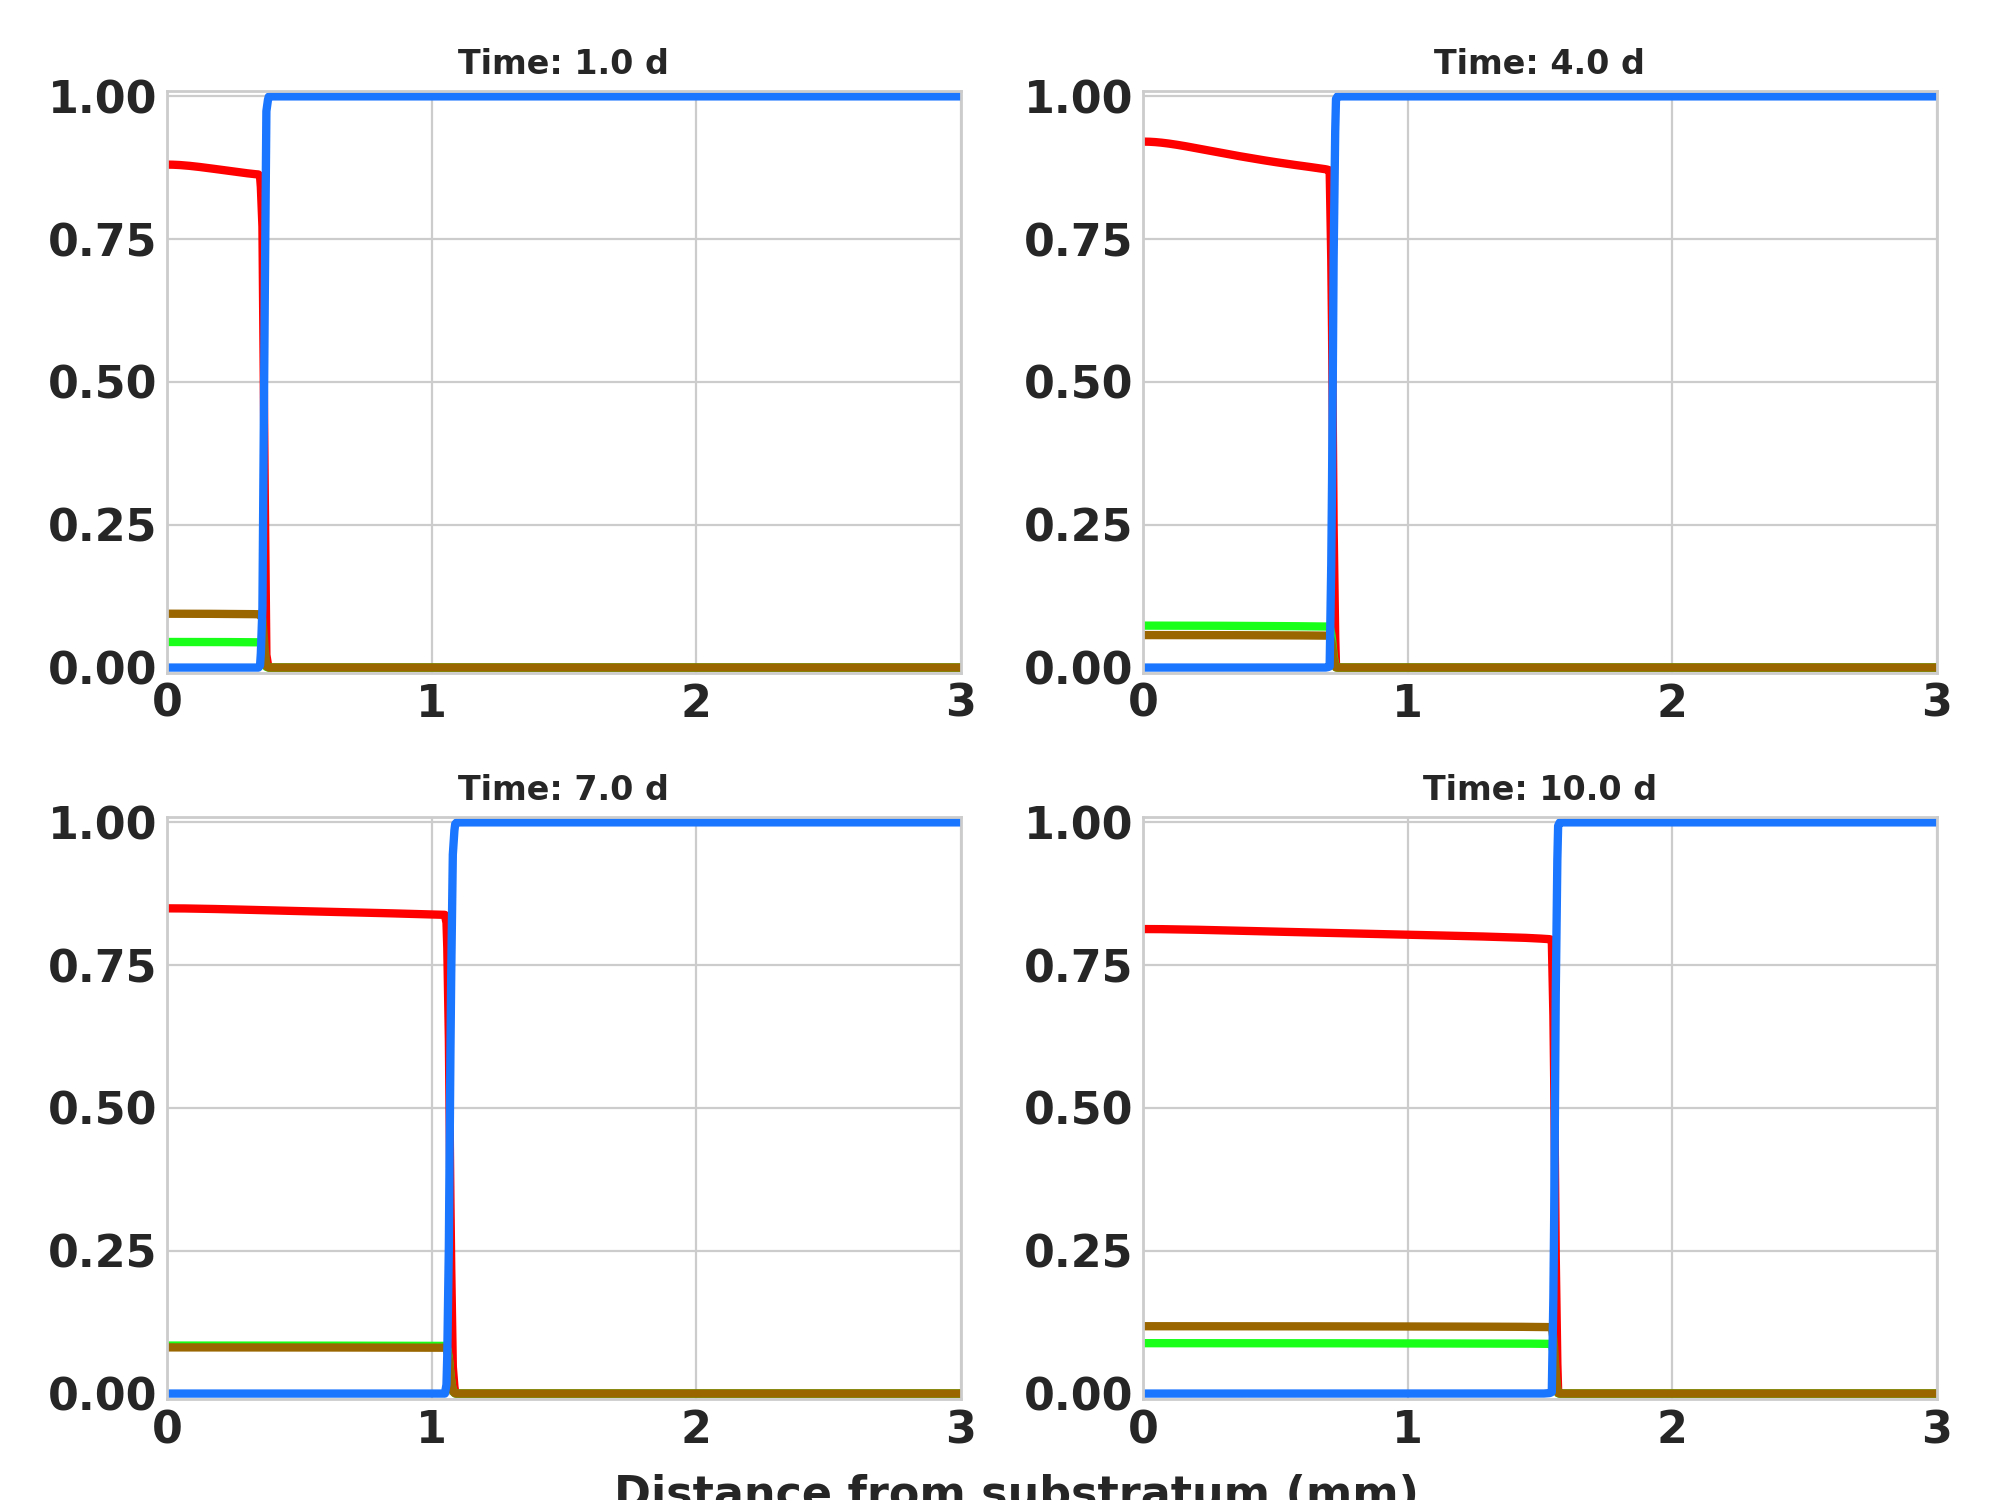
\includegraphics[width=\textwidth,height=0.45\textheight]{Chap4/methods/output/case5.png}
    \caption{Spatial distribution of particulates and water over domain height. Biofilm was initiated as a uniform biofilm over a substratum irradiated at 30 W m\textsuperscript{-2} at 850 nm.} 
    \label{fig:case5_dist_frac}
\end{figure}


\subsection{Case 5: Sparsely distributed biofilm irradiated from above}
The initial and boundary conditions for case 5 were identical for those used in case 4, however the radiative field was initialised from the top of the domain (at y = 3 mm). The purpose of this simulation was to assess whether there was a discernible difference in biofilm behaviour due to these different operating conditions. 

\begin{figure}[H]
    \centering
    \hspace*{-1cm}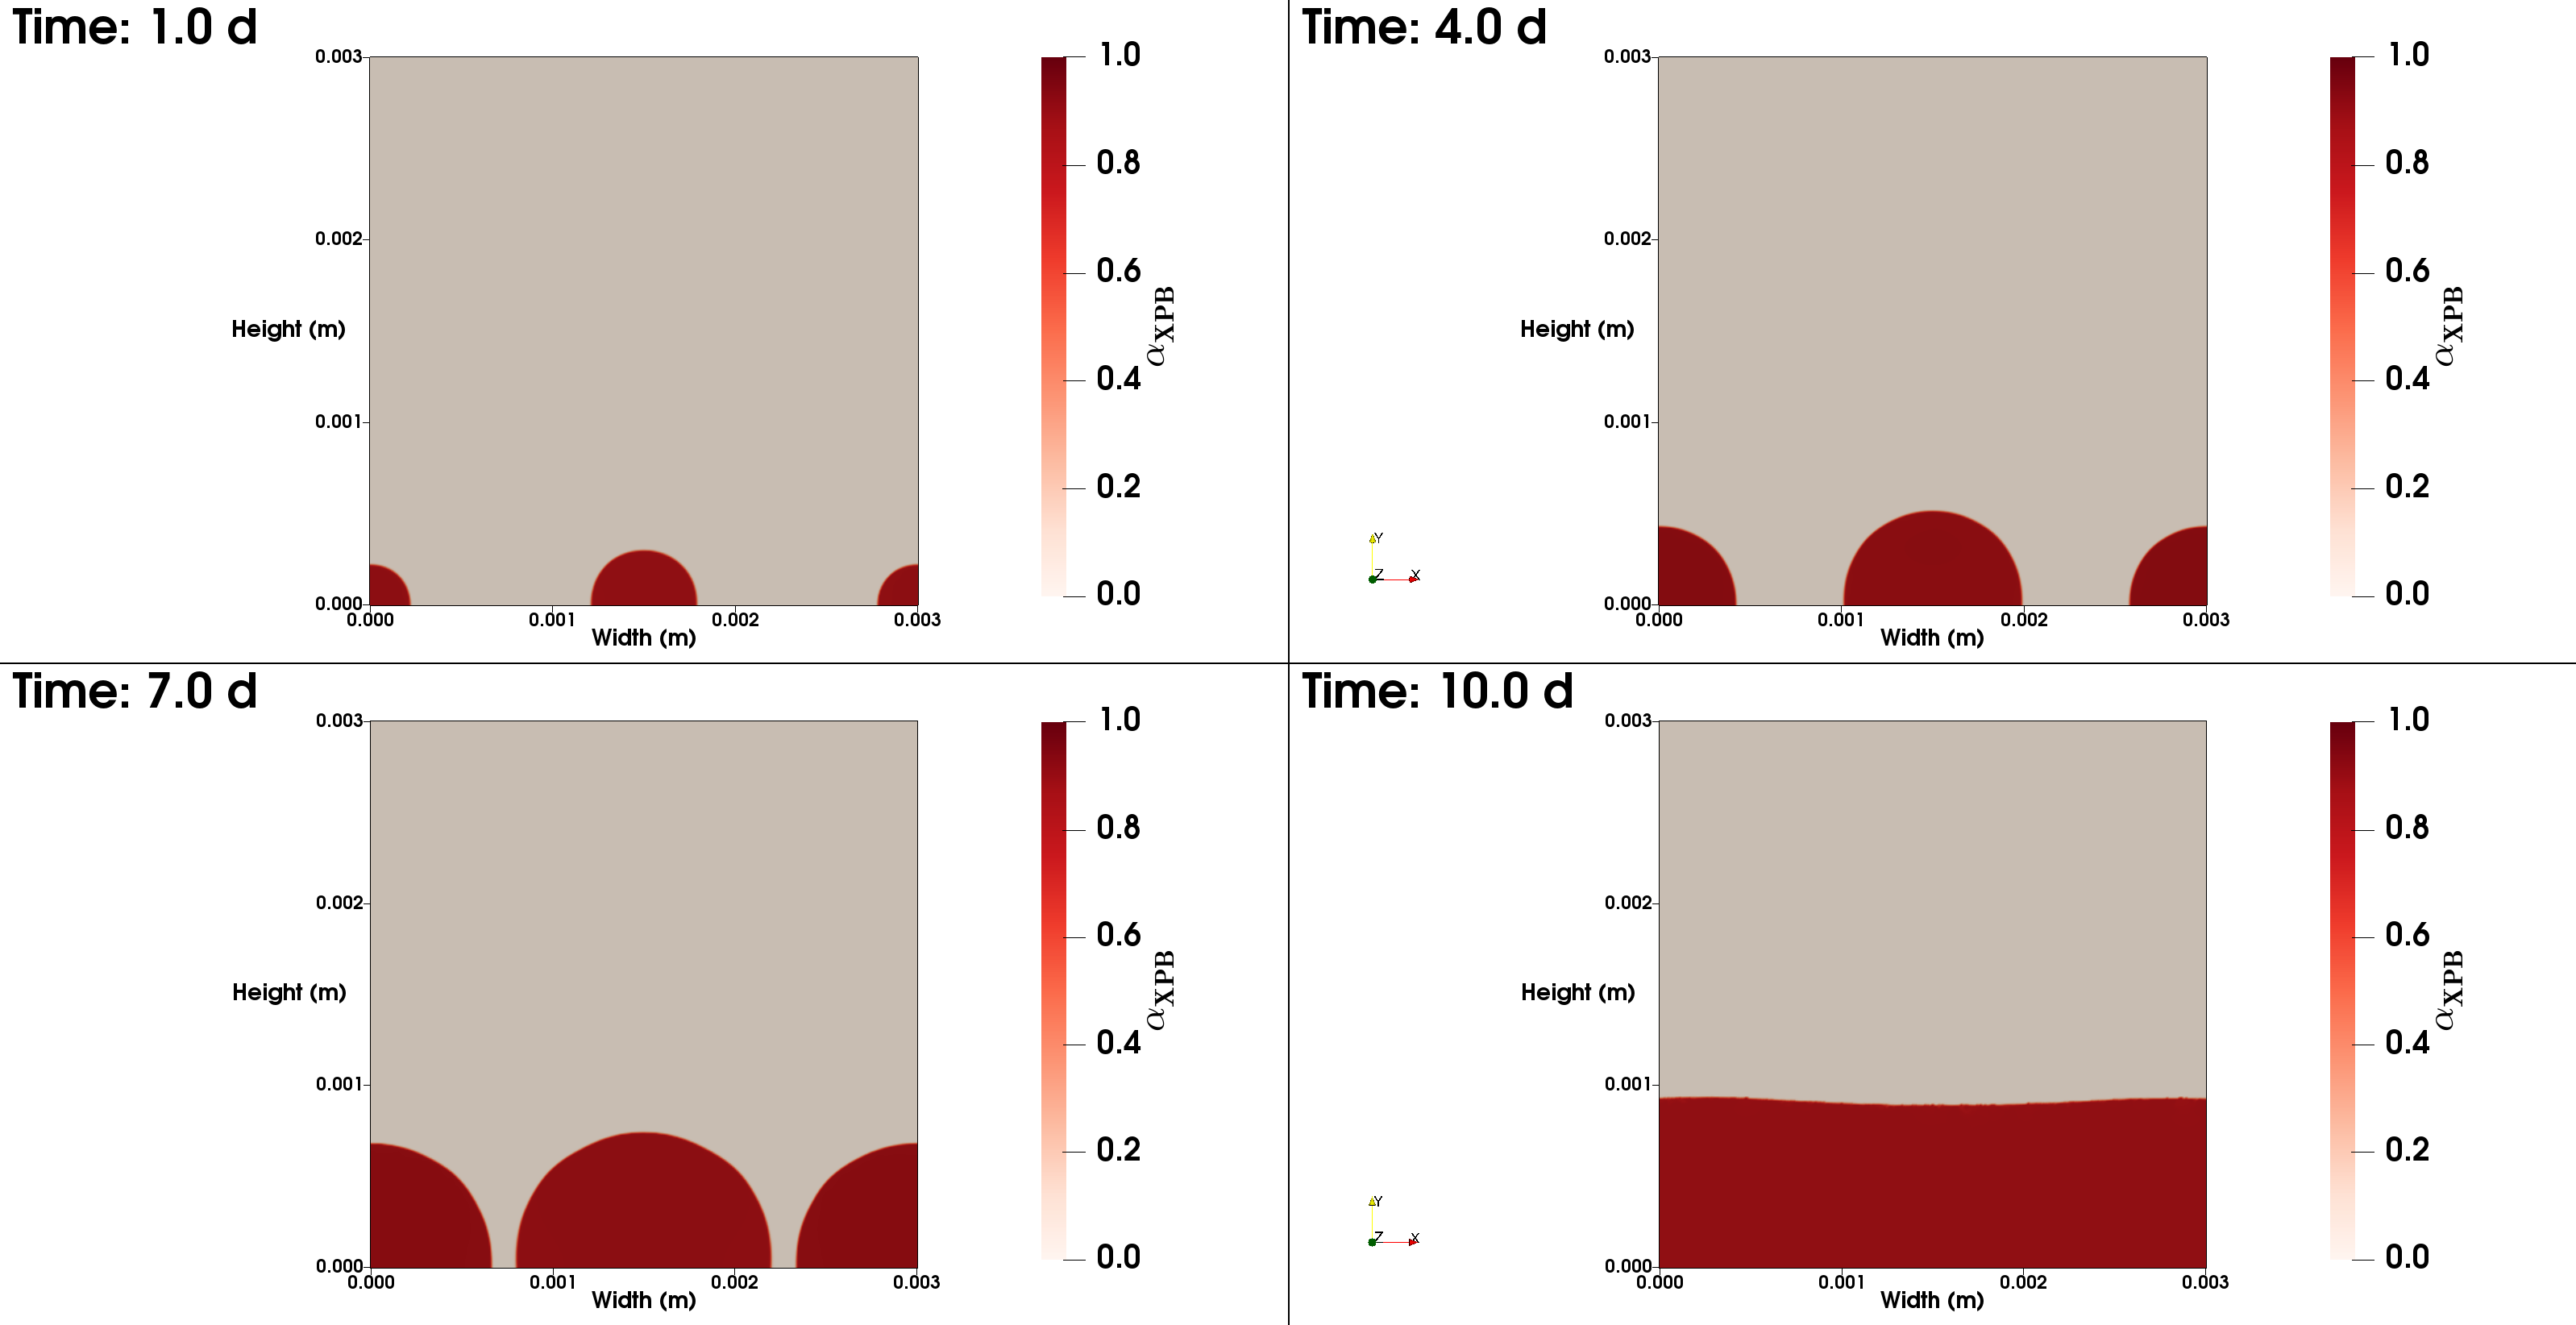
\includegraphics[width=1.1\textwidth,height=0.4\textheight]{Chap4/methods/data/figures/case6_ppb_frac.png}
    \caption{Two dimensional view of PPB as sparsely initiated biofilm irradiated from above at 30 W m\textsuperscript{-2} at 850 nm.} 
    \label{fig:case6_ppb_frac}
\end{figure}
There was considerably less biofilm formation over the 10 day period when compared with case 5 where the biofilm was irradiated from beneath the substratum. This indicates that despite limitations associated with diffusion being overcome, the radiative field limitation affects the growth of phototrophic at thicknesses on the order of 10\textsuperscript{-3} m, where scattering and absorption effects are more pronounced. The biofilm profile was also slightly different to the previous case, where the biomass was attracted to the light source, elongating the shape of the biofilm. As radiation is a condition for phototrophic growth, the biofilm tended to occupy and grow in the space where the radiative field was most intense. This was in along the x-y line where x was 1.5 mm. The higher intensity was due to the in-scattering phase function in the radiative transfer equation where the point with the most number of neighbours can attain the highest radiative intensity. 



\begin{figure}[H]
    \centering
    \hspace*{-1cm}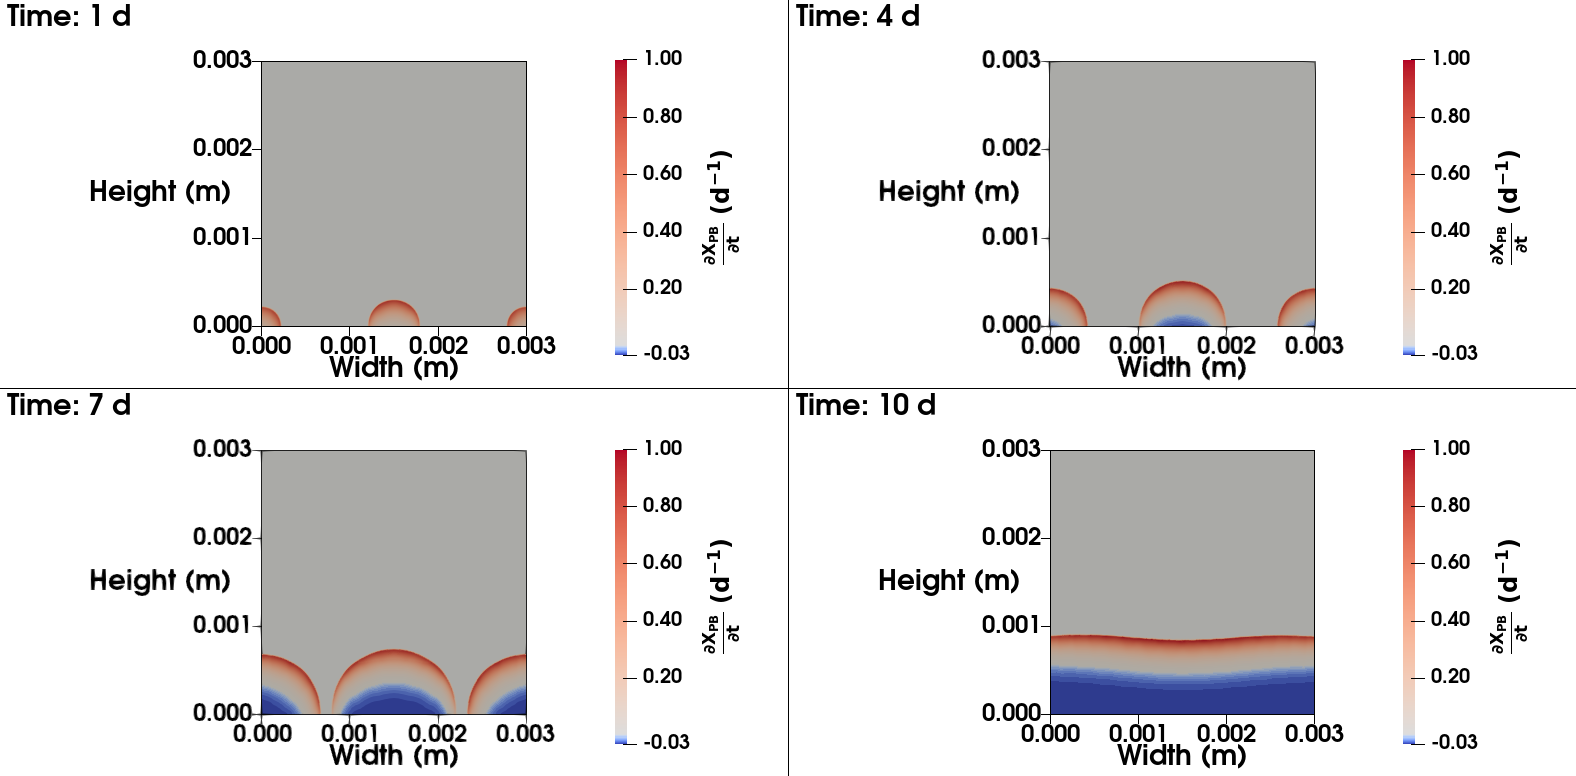
\includegraphics[width=1.1\textwidth,height=0.4\textheight]{Chap4/methods/data/figures/case6_growth_frac.png}
    \caption{Two dimensional view of PPB growth rate as sparsely initiated biofilm irradiated from above at 30 W m\textsuperscript{-2} at 850 nm.} 
    \label{fig:case6_growth_frac}
\end{figure}
The maximum apparent growth rate in this simulation is 1.0 d\textsuperscript{-1}. Phototrophic growth is positive until day 4, where the combination of self shielding and limiting diffusion lead to a negative growth rate in some regions on the substratum. The proportion of decaying biomass in the biofilm increases with time, as new biomass is created closer to the radiative source, shielding older biomass from sufficient light for growth. Additionally, as new biofilm occupies all the space along the substratum, diffusion limitations also have a greater contribution to the proportion of phototrophic biomass in decay mode. In a similar fashion to case 5, when clusters of biomass are present, the radiative field can more effectively reach the outer parts of the cluster despite the fact that they are further from the radiative source. This is due to the higher attenuation of the radiative field due to particulate matter when compared to water. This finding could not have been explored in a 1 dimensional simulation, as the spatial nature of the radiative field could not have been expressed. Therefore, due to the specific physical phenomena occurring in phototrophic biofilms compared with non-phototrophic organisms, expressing the behaviour in higher spatial dimensions is necessary in order to better understand these process limitations and overcome them when designing new phototrophic technologies.




\begin{figure}[H]
    \centering
    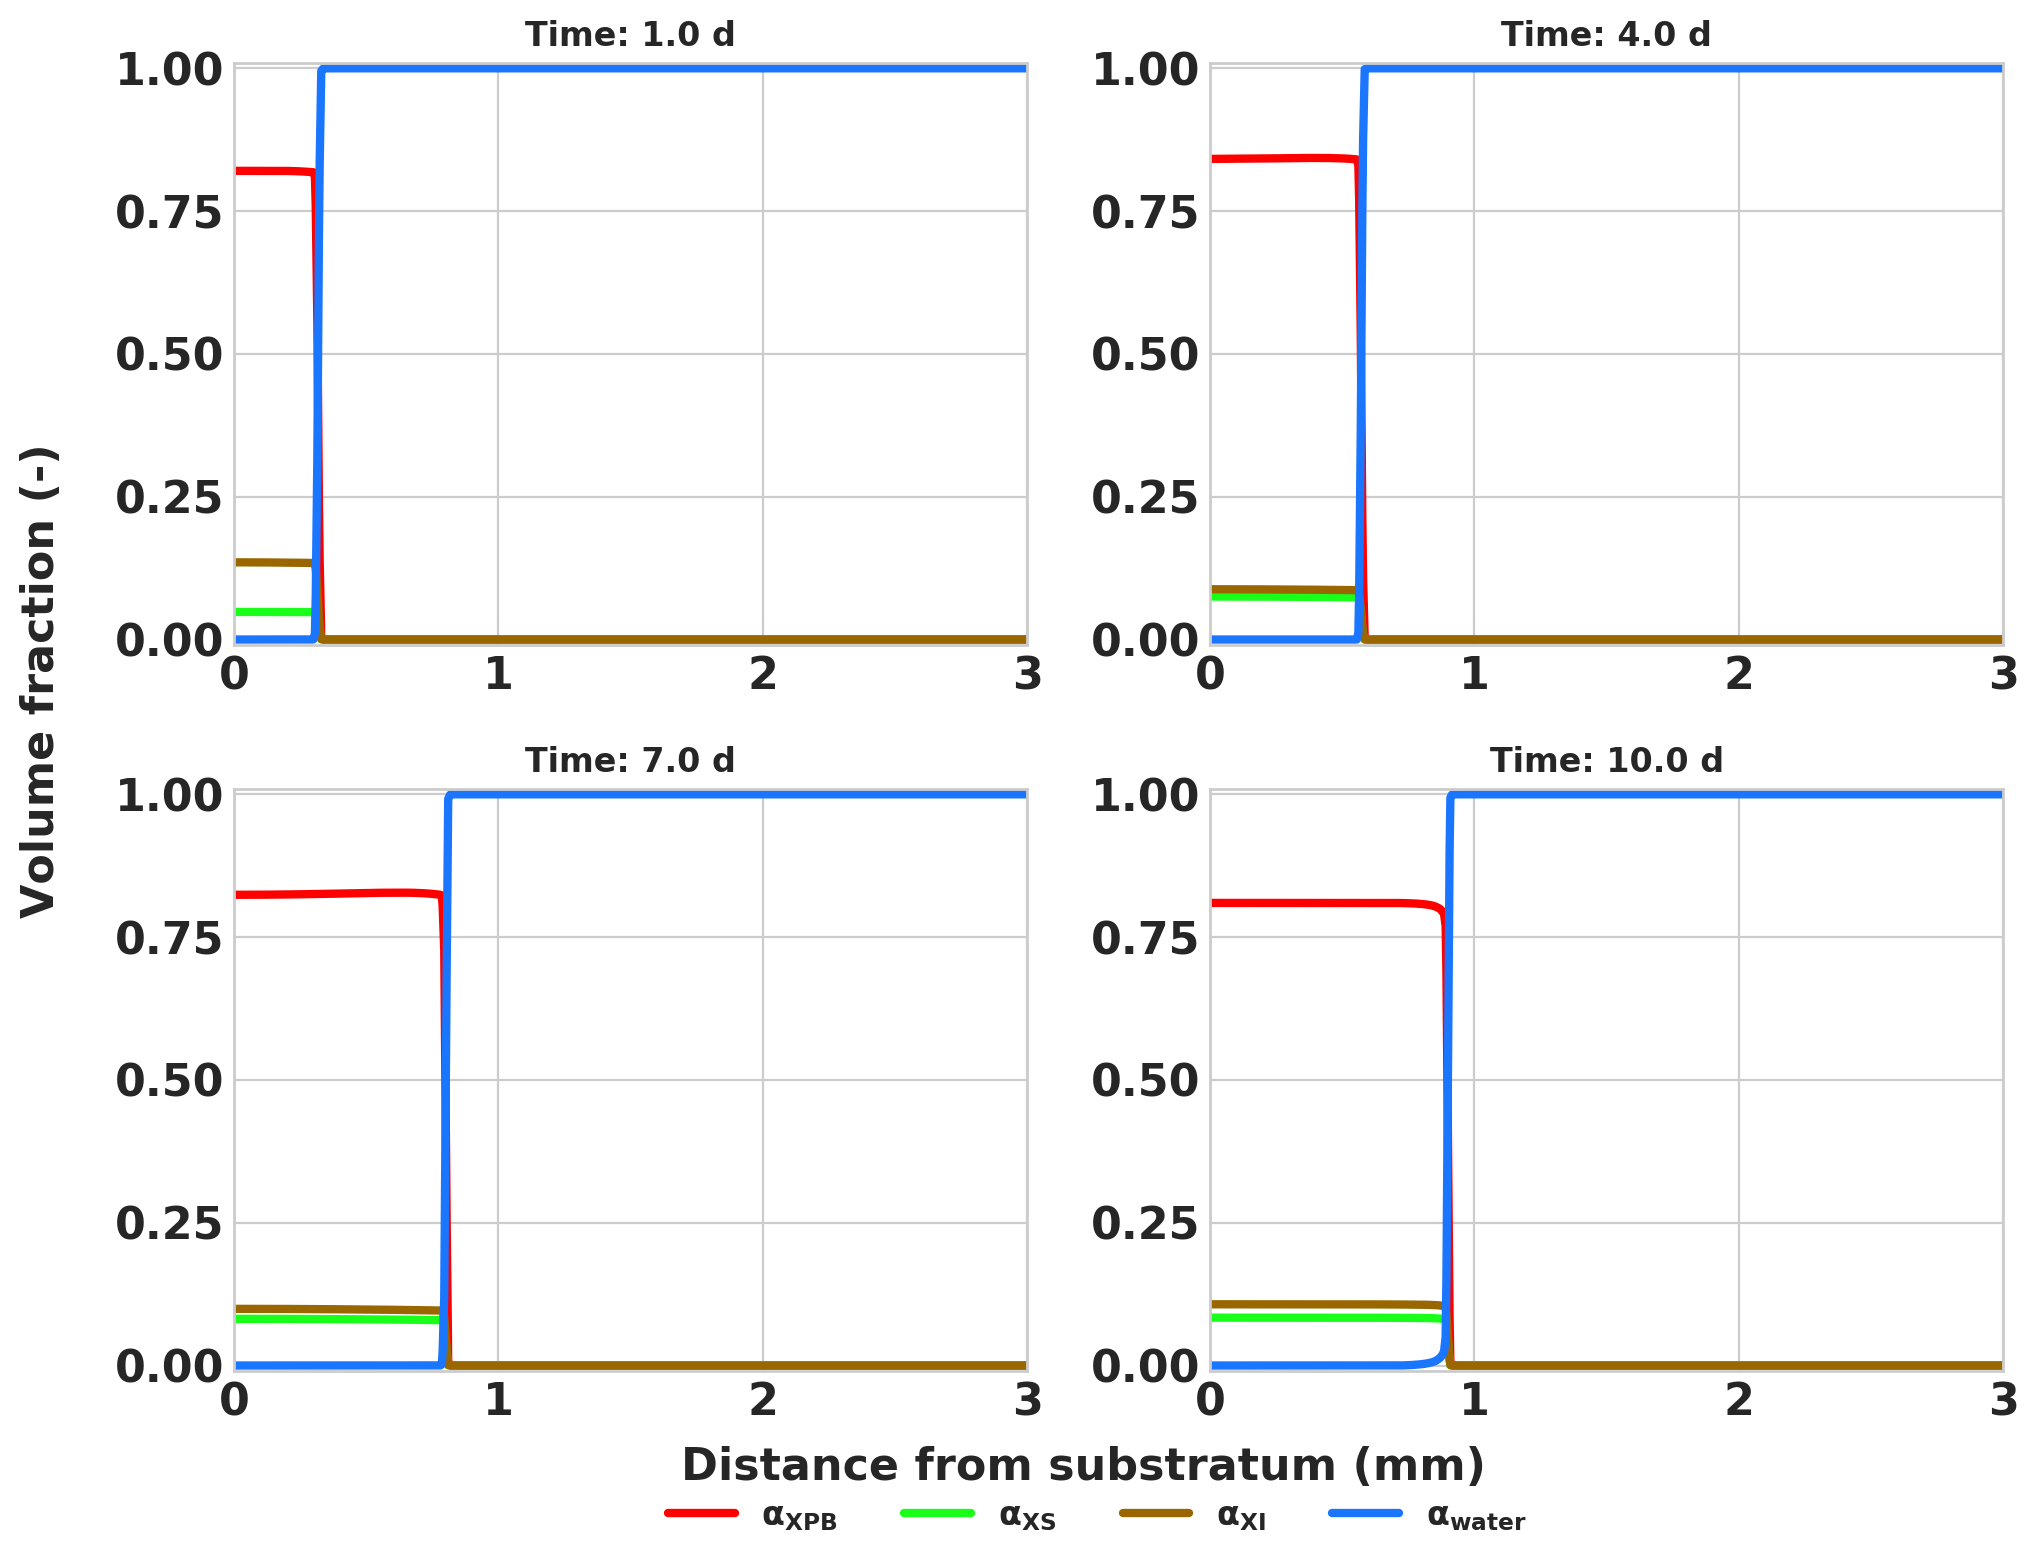
\includegraphics[width=\textwidth,height=0.45\textheight]{Chap4/methods/output/case6.png}
    \caption{Spatial distribution of particulates and water over domain height. Biofilm was initiated as a uniform biofilm irradiated from above at 30 W m\textsuperscript{-2} at 850 nm.} 
    \label{fig:case6_dist_frac}
\end{figure}

The biofilm distribution (Fig. \ref{fig:case6_dist_frac}) is relatively uniform throughout the domain. There is a slight increase along the height of the domain in PPB volume fraction when compared with case 5. This is due to the increasing intensity of the radiative field perceived by the biofilm front as it grows. 

\subsection{Case comparisons}

\subsubsection{Specific phototrophic activity}
After 10 days of growth, there were different specific phototrophic activities across the different test cases as show in Fig. \ref{fig:ch4_spa}. The case of low irradiance was omitted because the growth was essentially zero at the end of the 10 day period. For the two cases where the radiative field was initialised from below the substratum (Fig. \ref{fig:ch4_spa}a uniform initial biofilm and Fig. \ref{fig:ch4_spa}c sparse initial biofilm), the specific growth rate of phototrophic biomass was the same, as the biofilm had grown, spread, and reached a steady state by this point in the simulation. For the cases where the irradiance was initialised from above the domain (Fig. \ref{fig:ch4_spa}b uniform initial biofilm and Fig. \ref{fig:ch4_spa}d sparse initial biofilm), there was a slight difference in specific phototrophic activity at 10 days. The sparse biofilm had a specific phototrophic activity of 2.55 kgCOD m\textsuperscript{-3} d\textsuperscript{-1} whereas the growth of the uniform biofilm at this point in time was 2.45 kgCOD m\textsuperscript{-3} d\textsuperscript{-1}. This is essentially the same growth rate, and it can be concluded that the attenuation of the radiative field through water is minimally affected when compared to the contribution of the biofilm. 

\begin{figure}[H]
    \centering
    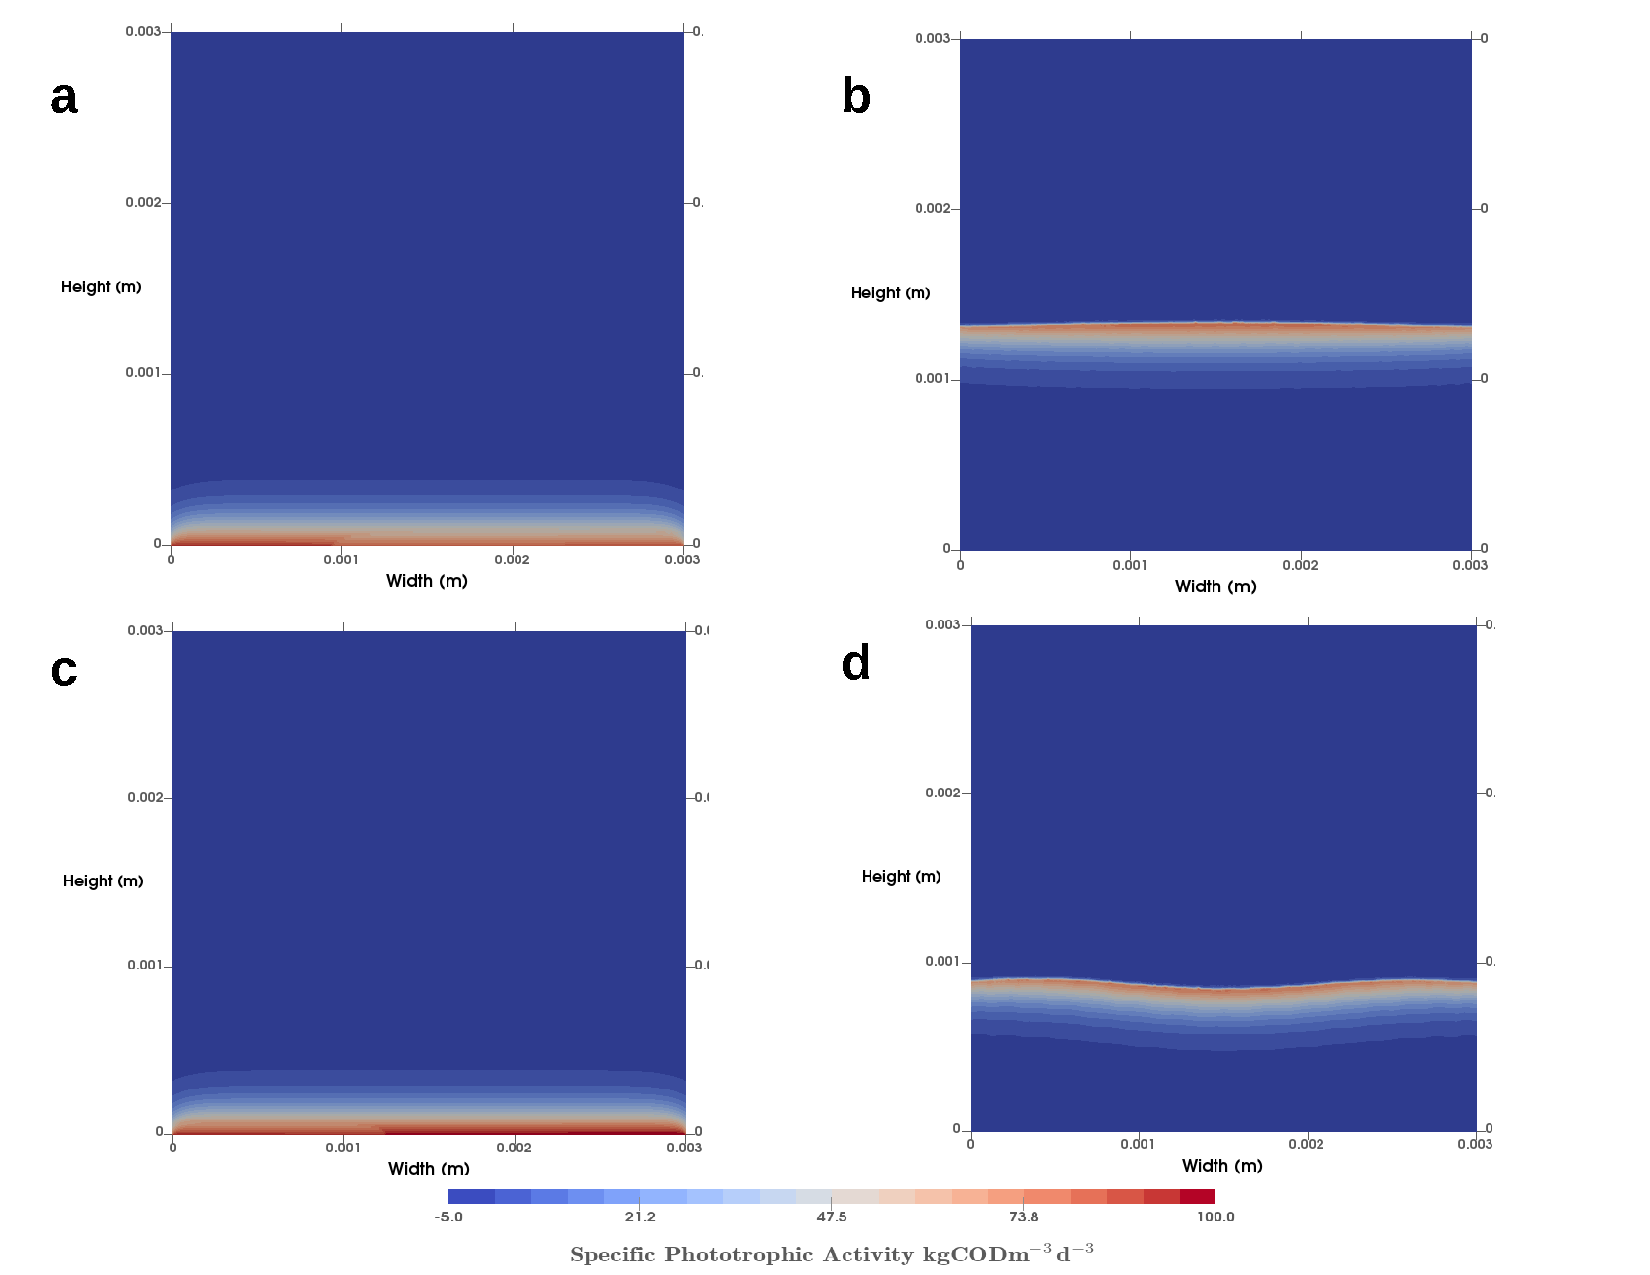
\includegraphics[width=\textwidth,height=0.5\textheight]{Chap4/results/post_processing/2D_cases/comparative/spa.pdf}
    \caption{Specific phototrophic activity distribution within the two dimensional domain at 10 days between a) case 1 with 30 Wm\textsuperscript{-2} irradiated from the substratum and a uniform initial biofilm, b) case 3 with a uniform initial biofilm and irradiance of 30 Wm\textsuperscript{-2} from above the domain, c) sparsely initialised biofilm with 30 Wm\textsuperscript{-2} irradiated from below the substratum, and d) sparsely initialised biofilm with 30 Wm\textsuperscript{-2} irradiated from above the domain.  } 
    \label{fig:ch4_spa}
\end{figure}

\subsubsection{Irradiance distribution after 10 days of growth}
As the growth rate of the biofilm and the radiative field are coupled, the spatial distributions of the radiative field support the conclusions from the specific phototrophic activity. Fig. \ref{ch4_rad10} shows the radiative field distribution for all cases excluding the case of low incident irradiance of 3 W m\textsuperscript{-3}. For the cases where the incident was from below the substratum, the irradiance follows roughly the same profile within the domain, with a small fraction experiencing any irradiance. This is the point from which the growth is driven, as was seen in Fig. \ref{fig:ch4_spa}. For both growth rate and irradiance distribution, the values for the uniformly initiated biofilm and the sparsely initiated biofilm (Fig. \ref{fig:ch4_rad10}a and Fig. \ref{fig:ch4_rad10}b respectively), the profiles are very similar at 10 days of simulated growth. This is due to a steady state being reached. As soluble substrates are supplied infinitely over time, this indicates that the limiting factor for growth in these biofilms is the radiative field. 

\begin{figure}[H]
    \centering
    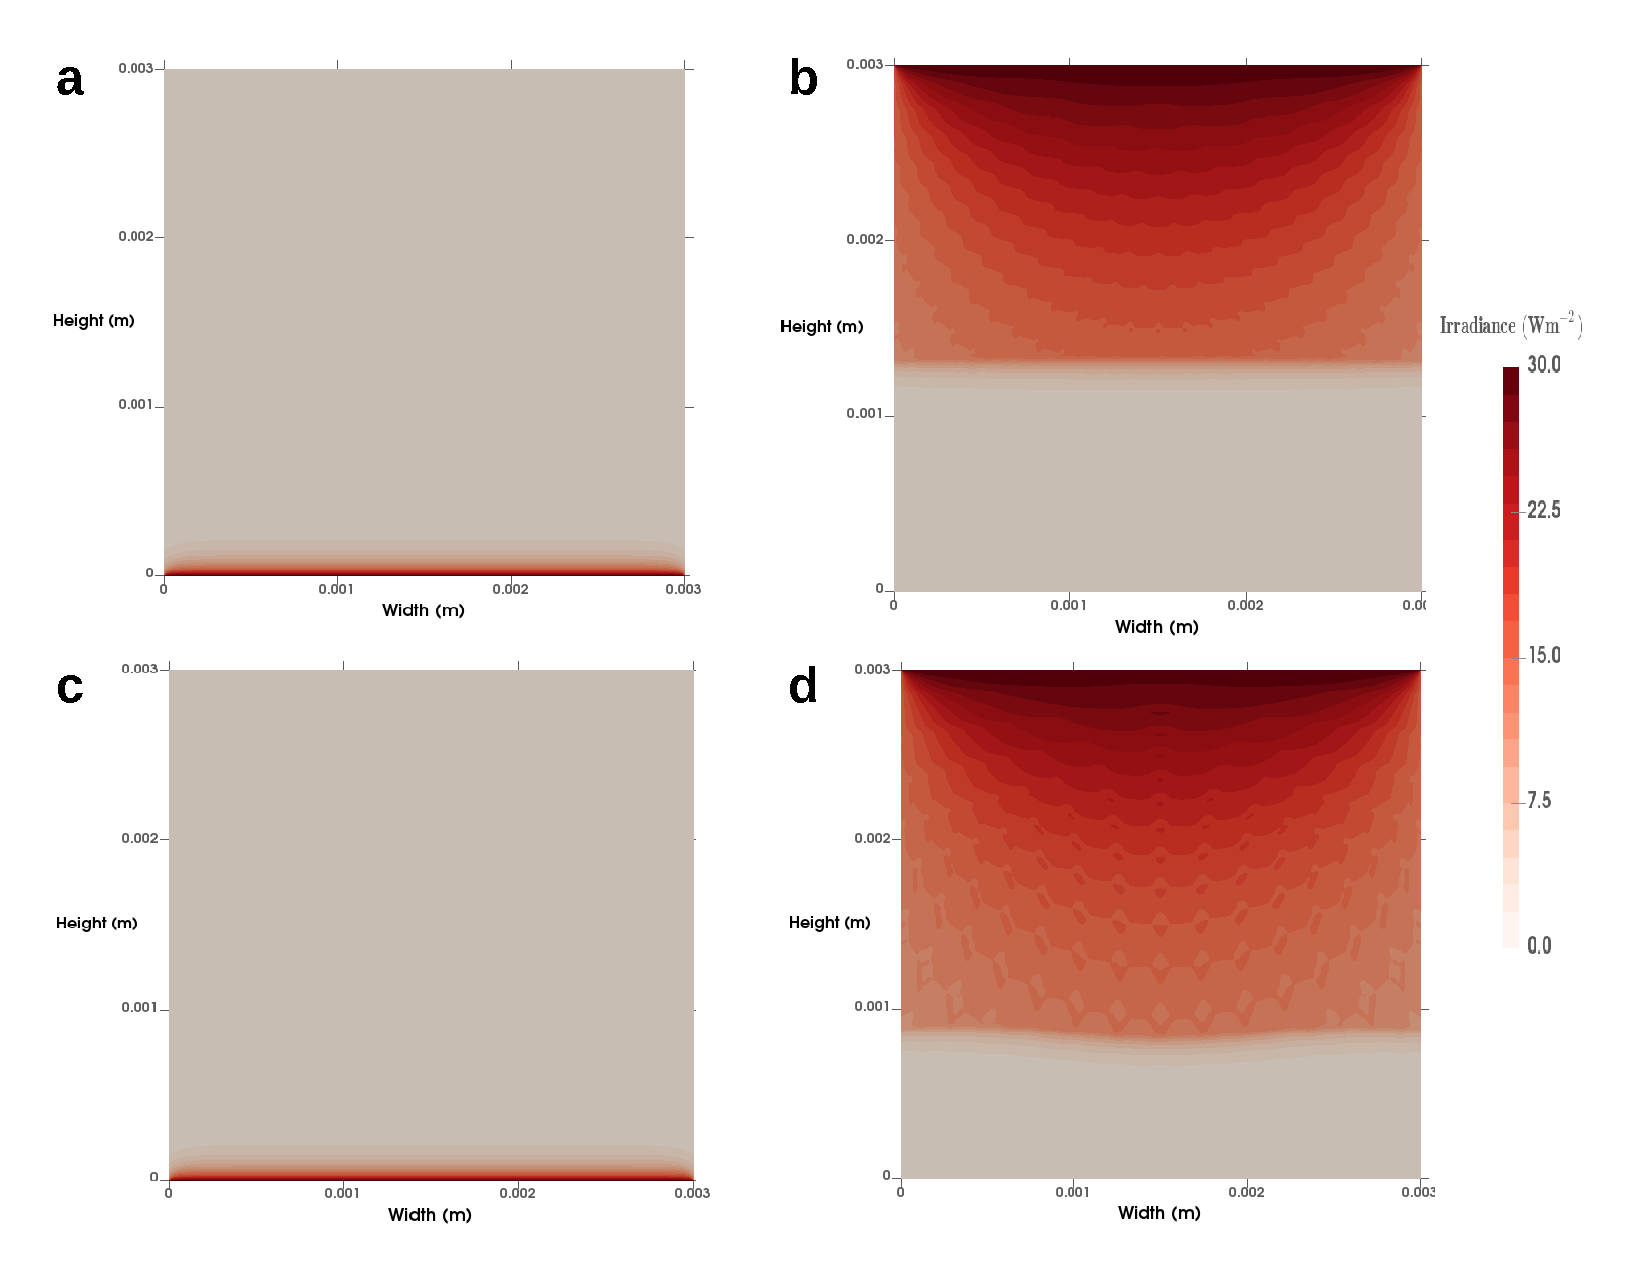
\includegraphics[width=\textwidth,height=0.5\textheight]{Chap4/results/post_processing/2D_cases/comparative/radiation.pdf}
    \caption{Irradiance distribution within the two dimensional domain at 10 days between a) case 1 with 30 Wm\textsuperscript{-2} irradiated from the substratum and a uniform initial biofilm, b) case 3 with a uniform initial biofilm and irradiance of 30 Wm\textsuperscript{-2} from above the domain, c) sparsely initialised biofilm with 30 Wm\textsuperscript{-2} irradiated from below the substratum, and d) sparsely initialised biofilm with 30 Wm\textsuperscript{-2} irradiated from above the domain.  } 
    \label{fig:ch4_rad10}
\end{figure}


\subsubsection{Volume averaged growth rate over time}
\begin{figure}[H]
    \centering
    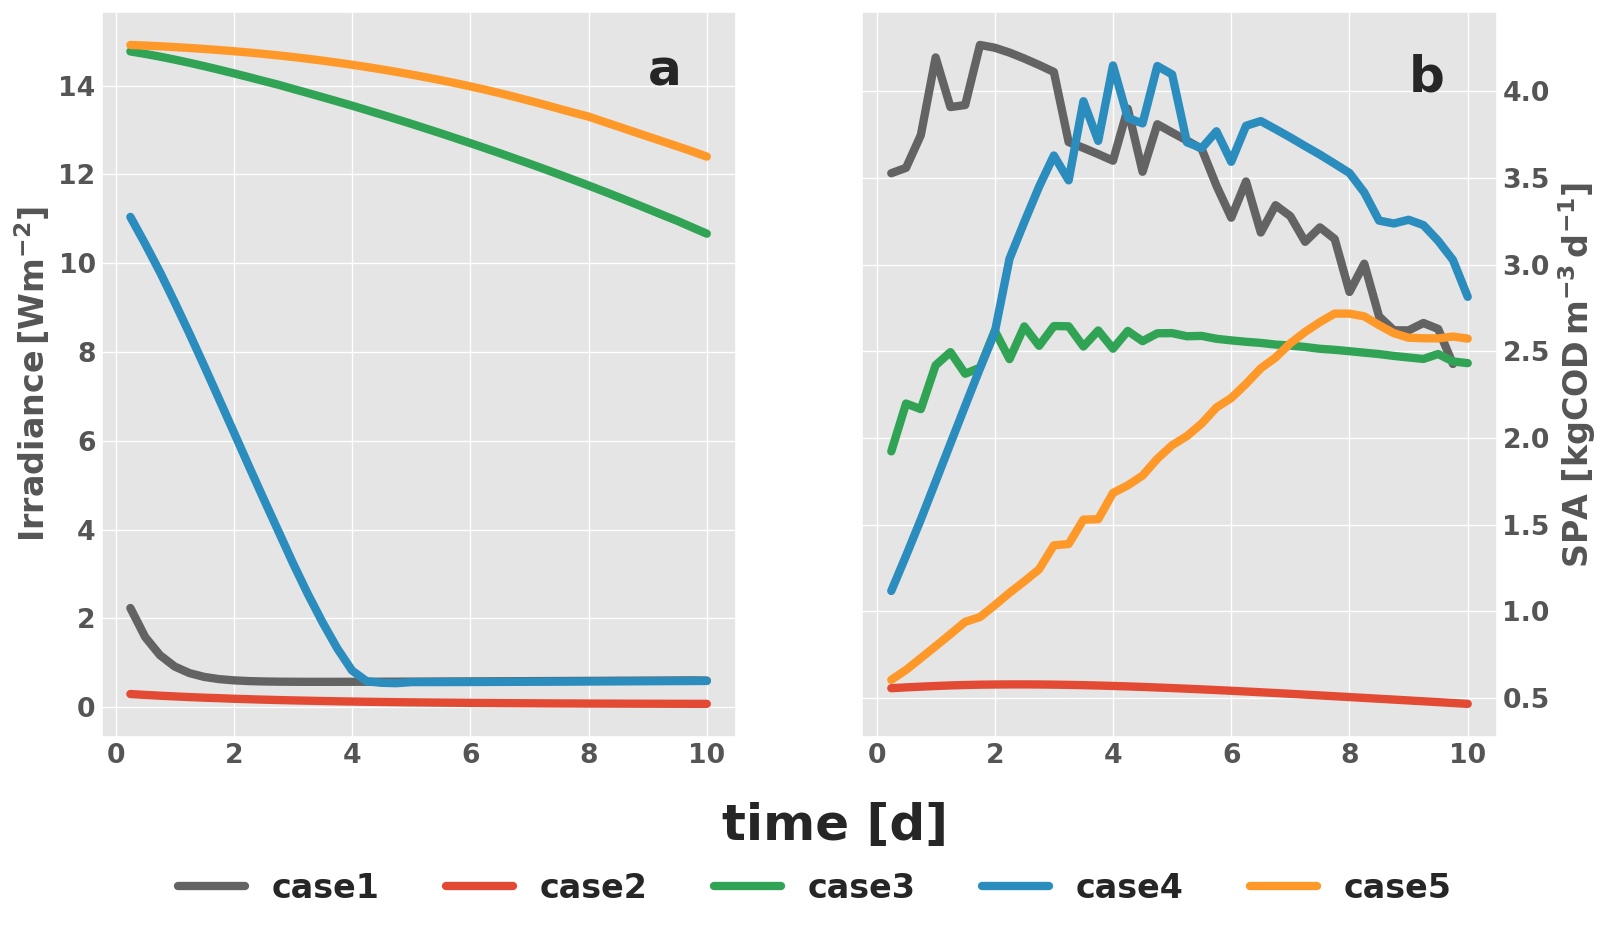
\includegraphics[width=\textwidth,height=0.3\textheight]{Chap4/results/post_processing/2D_cases/vol_averaged.png}
    \caption{Volume averaged irradiance for all cases at 850 nm irradiance (a) and specific phototrophic activity (b) over time.} 
    \label{fig:vol_averaged}
\end{figure}


%%%%%%%%%%%%%%%%%%%%%%%% DISCUSSION
\section{Analysis and model limitations}
In this study, a phototrophic biofilm model was developed using computational fluid dynamics methods (CFD). In this model, biomass growth and its coupling to a radiative field has been described, however there still exist some important aspects of the biofilm life-cycle which have not been developed in this work, but which merit discussion. The life-cycle of a biofilm includes the attachment of planktonic organisms to a substratum, growth and decay processes the microbial community, response to external hydrodynamic fields, and biofilm sloughing.
\skippingparagraph
In this study, it has been assumed that microorganisms have already found a point of attachment on a substratum, and there are no external planktonic microorganisms within the domain. Realistically, physical characteristics such as substratum roughness, cell surface, and current biofilm characteristics in relation to a planktonic cell in question all have an effect on the probability of cell attachment \cite{donlan2002}. Before any initialised biofilm, probabilistic functions based on substratum structure can be imposed for planktonic attachment. Some modelling has been done on the initial stages of biofilm formation, where planktonic microorganisms become attracted to sensing molecules of other organisms, and these sensing molecules have source or sink terms based on biofilm growth or attachment of planktonic biomass respectively \cite{moustaid2013}. The model was a continuum-based approach to biofilm modelling, with a biased random walk for the attachment of planktonic organisms to the biofilm. 
\skippingparagraph
The model for biofilm growth was accompanied by several assumptions. In order to convert the chemical oxygen demand (COD) quantities of the particulate species to volumetric expressions, cell water content, biofilm void fraction, and biofilm density were assumed. These values were all justified from literature values, but more refinement in selecting or calculating these values could lead to a more accurate biofilm growth model. In addition to the assumptions associated with volumetric biofilm expansion, the biokinetic model was developed using only one participating particulate species. In reality, and even more so in biofilm communities, there are myriad microorganisms each playing an important role within the biofilm matrix \cite{donlan2002}. Parameters such as substrate diffusion limitations or radiative field attenuation mean that phototrophic bacteria are most likely not the only living species within phototrophic biofilms. There are currently no phototrophic biofilm implementations which include non-phototrophic biomass as a state within the model, yet this would be a more precise representation of reality. The final limitation regarding biofilm growth is that the biokinetic model developed in Chapter 2 was for planktonic biomass, and due to the proximity and chemical signalling between other cells, biofilm organisms can display vastly different behaviour in the biofilm compared with their planktonic state. An experimental approach would therefore be required to calibrate and validate the biokinetic model. For the moment, the bounds of validity are assumed to hold for phototrophic biomass within a biofilm. 
\skippingparagraph
The final limitation regarding this phototrophic biofilm model is that an external flow field was not considered. Shear stress can have a significant influence on the structure and shape of biofilm \cite{donlan2002}, however with the efforts required to couple the volumetric growth to a radiative field, the influence of an external flow field has been left as an extension exercise. The inclusion of the coupled biofilm and flow field would not only paint a clear picture of the structure of the biofilm under stress, but would also present us with and understanding of how growth can be limited or minimised in cases where phototrophic biofilms are not desirable. 



%%%%%%%%%%%%%%%%%%% CONCLUSIONS
\section{Conclusions}
In this study, a multidimensional continuum-based phototrophic biofilm model was developed. The process of building the model included the translation of process biokinetics to volumetric growth, and the coupling of the radiative field to the volumetric biokinetic model, as was previously demonstrated in chapter 3. The solid and soluble species within the biokinetic model were simulated in a hybrid volume of fluid (VoF) and mixture model.
\skippingparagraph
%Five different simulations were done in order to explore the potential limiting factors of phototrophic biofilms. The five cases included: 1) sufficient soluble substrates and radiation (30 W m\textsuperscript{-2}) on a uniformly initialised biofilm, 2) limiting irradiance (3 W m\textsuperscript{-2}) with all other factors maintained, 3) sufficient soluble substrate with a radiative field initialised from above the biofilm, 4) a sparsely clustered biofilm with sufficient soluble substrates and radiation, and 5) the same as case 4, but with an overhead irradiance. 
\skippingparagraph
It was found that both the diffusion limitations of soluble substrate and the radiative field limited biofilm growth, however the radiative field was the main factor in restricted growth rates, due to the sometimes very localised field when biomass concentration was high. Biofilms with radiation above performed less well than those irradiated from below the substratum, most probably due to the non-uniformity and attenuation of the radiative field through water before reaching the biofilm front. 
The spatial differences of the radiative field led to the conclusion that models with dimensions higher than 1 are necessary in order to capture properly phototrophic growth.
\skippingparagraph
Several limitations were identified. The biokinetic model was only defined in terms of a single lumped phototrophic biomass, and it is hypothesised that an upgrade to the biokinetic matrix would be necessary to appropriately describe the spatially varying biofilm community, especially because a radiative field could lead to quite different communities within a biofilm matrix. There was no externally induced flow field which could have affected the growth and the eventual sloughing of biofilm, and this was highlighted as a point to improve for future iterations of the model. Finally, as organisms can express different genes and phenotype depending on whether they exist in biofilm or in planktonic state, an extensive laboratory study would be required to re-calibrate and validate this CFD model for phototrophic biofilm purposes.